\documentclass[ms,lof,lot]{metadata/cwru}
% \documentclass[[{phd}|masters],[lof],[lot],[copyright]]{cwru}

\title{Design Considerations for The Characterization of Capacitors}
\author{Michael L. DeLibero}
% Customize the type of document
%\CWRUdocumentname{Report}
% Customize the degree
%\CWRUdegree{Master of Science}
% Adds your advisor
\CWRUadvisor{Dr. Merat} 
\CWRUCommitteeOne{Gerhard Welsch}
\CWRUCommitteeTwo{Christian Zorman}

% The name of your department ("Department of" is added by the class)
\CWRUdepartment{Electrical Engineering\\ \& Computer Science}
\CWRUgraduationdate{January, 2016}
\CWRUdefensedate{July, 2015}

\pdfoptionpdfminorversion=7 %My schematic is being generated with pdf version 1.7
\usepackage{amsmath,amsthm,amssymb}
\usepackage{pdfpages}
\usepackage{comment}
\usepackage{multicol}
\usepackage{appendix}
\usepackage[framed,numbered,autolinebreaks,useliterate]{mcode}
\usepackage{nameref}
\usepackage[colorlinks,allcolors=black]{hyperref}
\usepackage[acronym,toc]{glossaries}
\usepackage{catchfilebetweentags}
\usepackage{tikz}
\usetikzlibrary{matrix,shapes,arrows,positioning,chains,calc,decorations.markings,fit}
\loadglsentries{metadata/glossaryEntries}
\bibliographystyle{plain}

\newif\ifisPPT
\isPPTfalse

\newcommand{\loadeq}[1]{%
   \ExecuteMetaData[./equations/equations.tex]{eq#1}%
}

\begin{document}

% Optional Sections 
\CWRUdedication{Dedication text}
\CWRUpreface{All portions of this master's thesis is the sole and original work of the author, Michael L. DeLibero, unless otherwise stated. 
Section: \ref{sec:history} \nameref{sec:history} is largely a compilation of other research and is cited as such. 
Section: \ref{sec:regression} \nameref{sec:regression} is an application of Levy's\cite{levy} and Sanathanan's\cite{levy_iter} work and is cited as such. 
The transimpedance amplifier seen in Appendix: \ref{app:schematic} \nameref{app:schematic} is largely based on previous work that I did with Steven Ehret which was published in his master's thesis \cite{steve_thesis}.

}
\CWRUack{I would like to thank my thesis advisor, Dr. Merat, for his support and instruction in helping me complete this work. I would also like to thank Dr. Welsch and ARPA-E, who's leadership and funding under ARPA-E contract DE--AR000016 made this work possible. Furthermore, I would like to thank Steven Ehret, who's initial work on this contract enabled my own.

}
%\CWRUloa{List of Abbreviations text}% Optional Glossary -- This is not complete
%\CWRUglossary{Glossary text}

% Required Abstract
\CWRUabstract{This thesis suggests a theoretical approach for characterizing capacitors at up to a 500VDC bias. A circuit design was developed that allows a user to characterize a capacitor via discharge curves and a swept frequency analysis of the impedance. An iterative, regression analysis is explored and then applied to capacitor modeling.
\label{sec:abstract}

}

% This must be run to generate all the preamble (Super \maketitle)
\CWRUpreamble{}

\section{Introduction}
\label{sec:intro}

This thesis presents a method to automate capacitor characterization in order to determine the physical differences between large numbers of research grade capacitors. It focuses on measuring capacitor characteristics through swept frequency analysis and discharge curve measurements in the presence of up to a $500V$ DC bias. The method then generates values for the physical parameters of the capacitors by fitting a model to the empirical data by applying a regression analysis.


\section {Background}

The following is a list of the questions that I will be answering in my background section.

\begin {enumerate}
    \item Where are capacitors used with a high DC bias?
    \begin {enumerate}
        \item What characteristics are the most important there?
        \item What are the main failure modes?
        \item What are the current specifications of the parts in use now?
        \item What research is being done to develop better capacitors for this use case?
        \item How do they currently evaluate the capacitors?
        \item How would they benefit from my research?
    \end {enumerate}
    \item What is the state of the art in capacitance measurement?
    \begin {enumerate}
        \item Impedance analyzers
        \item Capacitance bridges
        \item Hi pot testers
        \item What are the good and bad points of each of these technologies?
        \item Why do they not solve the problem that I stated? 
        \item Why does this technology not currently exist?
    \end {enumerate}
    \item What work has been done similar to this in the past?
    \item What are the important characteristics of capacitors?
    \item Is there any evidence that a capacitor's properties will change over DC bias?
\end {enumerate}


\section {Capacitor Parameters}
\subsection{Comments}
*In Section 3.1 you could mention what characteristics are important for that application.  And capacitors for switching power supplies are conspicuously absent.
*Do you want to get into capacitor parameters such as stability, temperature operating range, working voltage, peak or surge current, etc

\subsection{Practical Capacitor Uses}

Before getting into the individual capacitor parameters, I will explain some of the basic uses for capacitors. Each of the individual parameters will be important and have a direct effect on the uses described here. One should be careful to remember that any model consisting of the parameters listed in this section (and others) only describes an approximation of what is happening inside of a capacitor. Models and capacitor parameters will never be 100\% correct, but can be made with fairly high accuracy. As long as the designer understands the circumstances in which the models are accurate, he can use them to make a better circuit.

The most basic reason for wanting to use a capacitor is that it has the ability to store charge, which is close to the same thing as saying that it has the ability to store energy. It can store and release energy quickly to be able to react to the needs of the circuit.

\subsubsection{Power Supply Bypassing}
\begin{figure}[ht!]
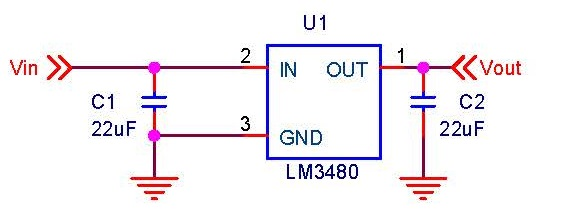
\includegraphics[keepaspectratio=true,scale=.5]{./figures/parameters/bypass.jpg}
\centering
\caption{Power Supply Bypassing Circuit}
\label{bypass}
\end{figure}

One of the most common uses of capacitors in bypassing a DC power supply (See Figure: \ref{bypass}). Without a bypass capacitor, a portion of the noise or any voltage spikes on the input to a power supply is passed to the output. A capacitor from the input to ground acts as a local charge reservoir to smooth out any non-DC components on the input voltage. Putting a bypass capacitor on the output of a supply prevents load surge currents from causing the output voltage to dip. This is especially important with digital chips, as their high frequency switching can result in glitching if the supply is not properly bypassed.


\subsubsection{Analog Filtering}

Another use for capacitors is in analog filtering. Take for instance the low pass figure in Figure: \ref{lowPass}. The capacitor is used in this configuration to control which frequencies get passed to the rest of the circuitry. Low pass filters are needed in many application; a few of them being anti-aliasing, clock filtering, and integration.

\begin{figure}
    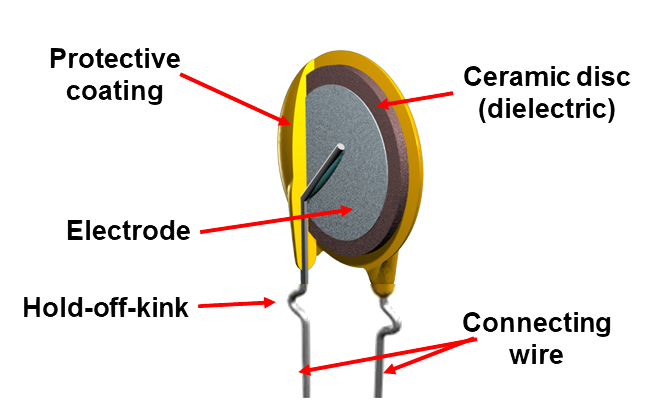
\includegraphics[keepaspectratio=true,scale=.5]{./figures/testImage.png}
    \centering
%    \cite{capSite_df_vs_temp}
    \caption{Low Pass Filter}
    \label{lowPass}
\end{figure}

\subsubsection{DC Blocking}

Designers often take advantage of capactors' characteristic of passing AC current while blocking DC current. As in Figure: \ref{dcBlock}, a capacitor can be used to block a DC offset before an amplifier. 

\begin{figure}
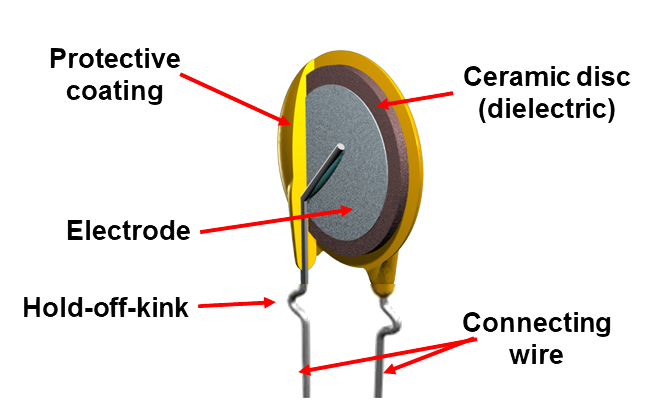
\includegraphics[keepaspectratio=true,scale=.5]{./figures/dcBlock.png}
\centering
%    \cite{capSite_df_vs_temp}
\caption{Using a capacitor in a DC blocking application}
\label{dcBlock}
\end{figure}



\subsubsection{Power Factor Correction}

The inductors in modern DC-DC switching supplies have required increased attention to the engineering phenomenon know as power factor. Any electrical load with an inductive component causes the supplied current phase to lag the voltage phase. This effect decreases the efficiency of the power distribution and also has the ability to cause stability issues. A capacacitor can be used as a simple, passive way to move the power factor back towards the ideal state (See Figure: \ref{powerFactor}). \cite{cui_powerFactor}
\begin{figure}[ht!]
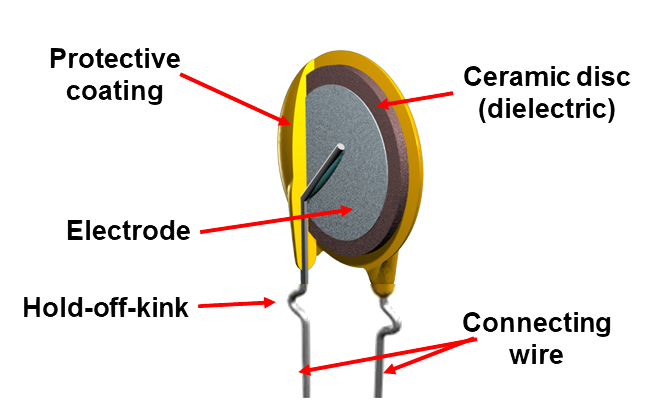
\includegraphics[keepaspectratio=true,scale=.5]{./figures/parameters/powerFactor.png}
\centering
\caption{Power Factor Correction Circuit}
\label{powerFactor}
\end{figure}



\subsubsection{Oscillators}
Capacitors are also used in oscillator circuits. -- Add resonator from HnH.

\subsection{Capacitance}

There is a distinct difference between a capacitor and capacitance. While a capacitor's main characteristic is capacitance, it cannot be modeled entirely as such in most practical applications. There are various inductive and resistive components to a capacitor that are important in various circumstances.

\begin{equation}
\label{cqv}
C=\frac{Q}{V}
\end{equation}

Capacitance is the ability to store electrical charge. Equation: \eqref{cqv} says that capacitance is stored charge that is spread throughout a volume. A device that can store a lot of charge in a small area has a large capacitance.The basic equation for a commercial capacitor is seen in Equation: \eqref{parPlateCap}.

\begin{equation}
\label{parPlateCap}
C = \frac{\epsilon _0 A}{d}
\end{equation}

When using a capacitor in a single-pole low-pass filter, the cutoff frequency can be determined by Equation: \eqref{lpfilter_eqn}. The circuit designer will choose a value for C and R in order to meet the cutoff frequency restraint.

\begin{equation}
\label{lpfilter_eqn}
f = \frac{1}{2\pi RC}
\end{equation}

Varying the capacitance used in the filter will move the cutoff frequency and consequently get a different response in the filter. The effect of this can be seen in Figure: \ref{lowPassFilt_fig}.

\begin{figure}
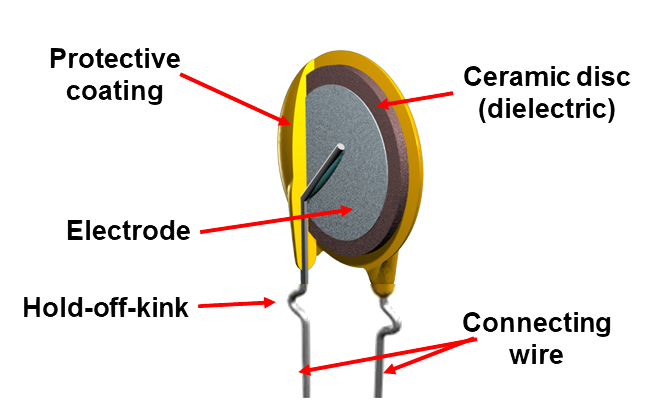
\includegraphics[keepaspectratio=true,scale=.5]{./figures/testImage.png}
\centering
%    \cite{capSite_df_vs_temp}
\caption{Changing Capacitance in a Low Pass Filter}
\label{lowPassFilt_fig}
\end{figure}

\subsection{Impedance}

The impedance of a capacitor is the "AC resistance" of the device. It determines the AC current that will flow when an ac voltage is applied to the capacitor via Ohm's law (Equation: \eqref{capOhmsEqn}). An ideal capacitor has no resistive elements and is purely capacitive. Therefore, its impedance can be described via Equation: \eqref{capImpEqu}. The two main things to notice are that the impedance is frequency dependent and it is purely imaginary (reactive).

\begin{equation}
\label{capOhmsEqn}
\vec{V} = \vec{I} \vec{Z}
\end{equation}

\begin{equation}
\label{capImpEqu}
\vec{Z} = \frac{1}{2\pi jfC}
\end{equation}

\begin{equation}
\label{capMagEqn}
Z = |\vec{Z}| = \frac{1}{2\pi fC}
\end{equation}

In most AC applications we look at the magnitude of the impedance. Real capacitors have a more complicated impedance, but with an ideal capacitor we can simplify the magnitude equation down to Equation \eqref{capMagEqn}

When capacitors are used in bypassing power supplies, the idea is to have a low impedance for common or expected noise frequencies. One may be tempted to choose a large valued capacitor to use for bypassing a wide range of frequencies. This turns out to backfire in practical situations, due to other parasitics in a real capacitor. For any capacitor, the impedance equation is more complicated, and the impedance value will begin to increase with frequency after some point. This will cause the designer to choose several different valued capacitors in parallel when bypassing a power supply or sensitive component. We will see later that the frequency plot of a capacitor will end up being more complicated than the simplified version seen in Figure: \ref{idealCapMagfig}.

\begin{figure}
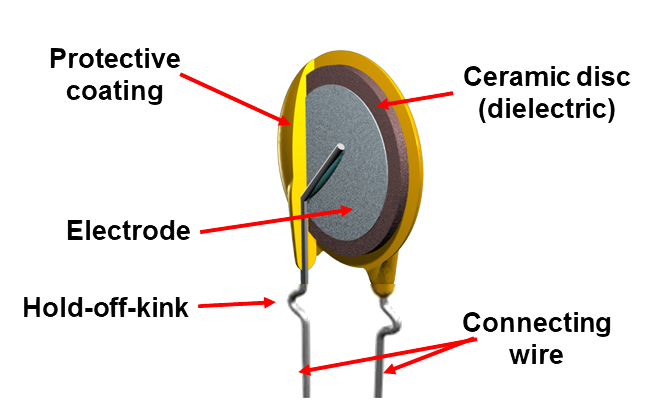
\includegraphics[keepaspectratio=true,scale=.5]{./figures/testImage.png}
\centering
%    \cite{capSite_df_vs_temp}
\caption{Ideal Capacitor Magnitude versus frequency}
\label{idealCapMagfig}
\end{figure}

\subsection{Phase}

The phase of a combination of resistive and reactive components can be written as in Equation: \eqref{capPhEqn}.

\begin{equation}
\label{capPhEqn}
\phi = tan^{-1}[\frac{X_c}{R_c}]
\end{equation}

For an ideal capacitor, having no resistance and only capacitance, the phase angle is only written as:

\begin{equation}
\label{capImpEqu2}
\phi = -i = -90^0
\end{equation}

The practical implication of this can be seen in the phase response of a low pass filter (Figure: \ref{lpFiltPhaseFig}). The capacitor introduces a phase lag relative to the input signal's frequency. If you would compare the input and output signals in time, the output's peak would lag behind the input's by the phase amount predicted in the phase response.

\begin{figure}
    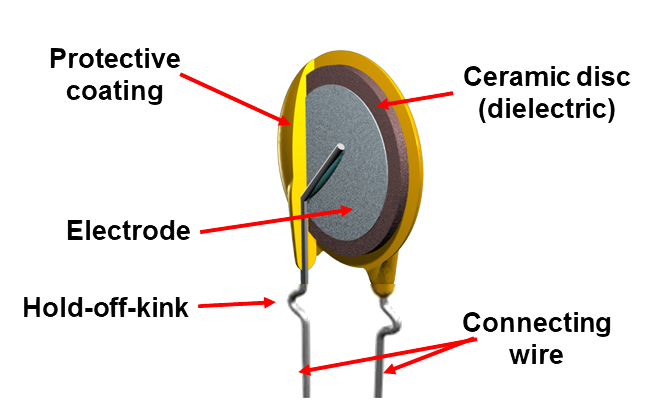
\includegraphics[keepaspectratio=true,scale=.5]{./figures/testImage.png}
    \centering
%    \cite{capSite_df_vs_temp}
    \caption{Low-Pass Filter Phase}
    \label{lpFiltPhaseFig}
\end{figure}

\subsection{ESL}

The Equivalent Series Inductance (ESL) of a capacitor is a lumped estimate of all of the inductive components of a capacitor. It is typically modeled as an inductor in series with the bulk capacitance (See Figure \ref{capESLModelFig}).

\begin{figure}
    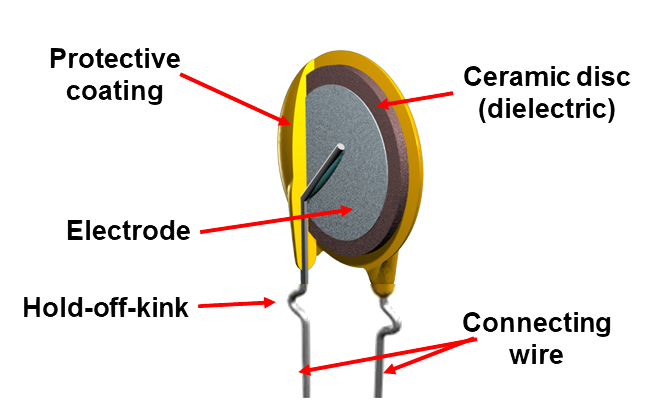
\includegraphics[keepaspectratio=true,scale=.5]{./figures/testImage.png}
    \centering
%    \cite{capSite_df_vs_temp}
    \caption{Capacitor ESL Model}
    \label{capESLModelFig}
\end{figure}

Adding ESL to the capacitive model creates a new impedance equation (Equation: \eqref{impESL}). Note that for L\textless \textless C, this equation simplifies to Equation: \eqref{capImpEqu} for low frequencies.

\begin{equation}
\label{impESL}
\vec{Z_c} = \frac{1-\omega ^2CL}{j\omega C}
%\cite{maxSwEff}
\end{equation}

\begin{equation}
\label{phaseESL}
\phi = Phase
%\cite{maxSwEff}
\end{equation}

Similarly, Equation: \eqref{phaseESL} shows that the phase of the capacitor is also affected at higher frequencies

\begin{figure}
    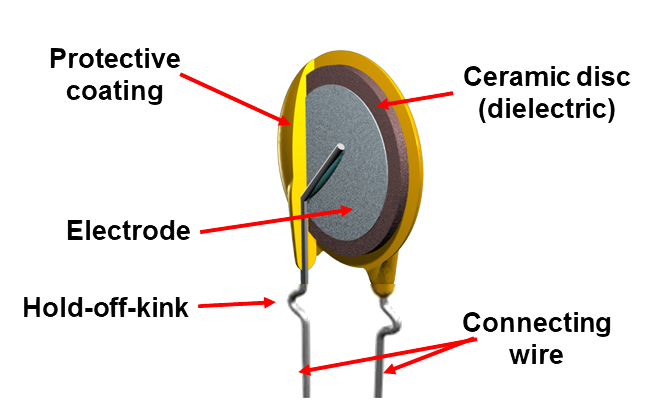
\includegraphics[keepaspectratio=true,scale=.5]{./figures/testImage.png}
    \centering
%    \cite{capSite_df_vs_temp}
    \caption{ESR+ESL Impedance-Phase Plot}
    \label{capESLPlot}
\end{figure}

Figure: \ref{capESLPlot} shows a graphical representation of a capacitor's magnitude and phase once ESL is considered. This plot shows that at a certain frequency, a capacitor's impedance will begin to increase with frequency. This means that a bypass capacitor will only be effective up to a certain frequency. Typically, the this frequency point and the capacitor's value have an inverse relationship. This is why you will see power supplies and sensitive chips being bypassed by a range of widely different valued capacitors. 

\subsection{ESR}
A real capacitor is more complicated than the ideal single capacitor model. One of the most used parameters is the Equivalent Series Resistance (ESR). ESR is the practical result of the fact that the materials used to create the capacitor have resistance. In simple cases, this can be approximated by a resistance in series with a capacitor (See figure: \ref{capESRModelFig}).

\begin{figure}
    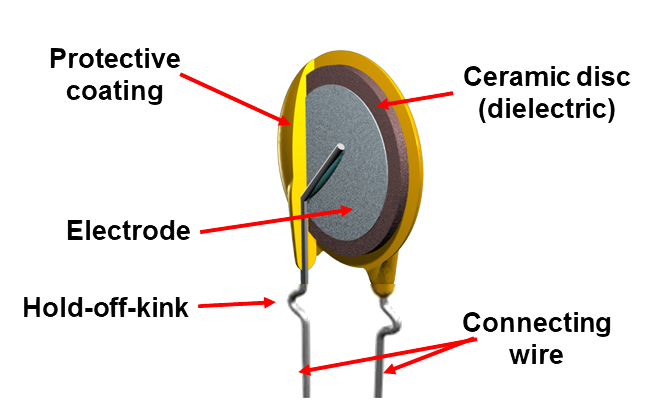
\includegraphics[keepaspectratio=true,scale=.5]{./figures/testImage.png}
    \centering
%    \cite{capSite_df_vs_temp}
    \caption{Capacitor ESR Model}
    \label{capESRModelFig}
\end{figure}

ESR becomes is important when thinking about DCDC switch mode power supplies. The converter's output voltage will have some ripple voltage on top of the DC output. This produces a ripple current through the capacitor. The capacitance element experiences no losses, but the ESR dissipates power according to Equation: \eqref{dcdcESReqn}

\begin{equation}
\label{dcdcESReqn}
P_{ESR} = I_{C,RMS}^2 * ESR
\cite{maxSwEff}
\end{equation}

\begin{equation}
\label{ImpCEslEsr}
\vec{Z_c} = ESR + j * (\omega L - \frac{1}{\omega C})
\cite{maxSwEff}
\end{equation}

Another important thing to note about ESR is that even though it is modeled as a resistance, it is not constant across all frequencies. It is a simplification of resistive and capacitive elements in a capacitor that are dominated by resistance.

\subsection{Resonance Frequency}

Once C, ESL, and ESR are included into the capacitor model, a parameter know as the self-resonant frequency becomes evident. Equation: \eqref{ImpCEslEsr} shows that when $Z_{ESL} == Z_C$, the capacitor is at its resonance point. At this frequency, the capacitor's impedance is determined solely by the ESR at that frequency. This frequency can be calculated by Equation: \eqref{fres}.

\begin{equation}
\label{fres}
f_r = \frac{1}{2\pi \sqrt{LC}}
\end{equation}

\subsection{Dissipation Factor}

Dissipation factor, otherwise known as the loss-tangent, is a measure of the energy stored to the energy dissipated per cycle. It is a measurement of the efficiency of the capacitor. The DF can be quantified through Equation: \eqref{dispFac}. 

\begin{equation}
\label{dispFac}
D = \frac{ESR}{Xc}
\end{equation}

\begin{figure}
    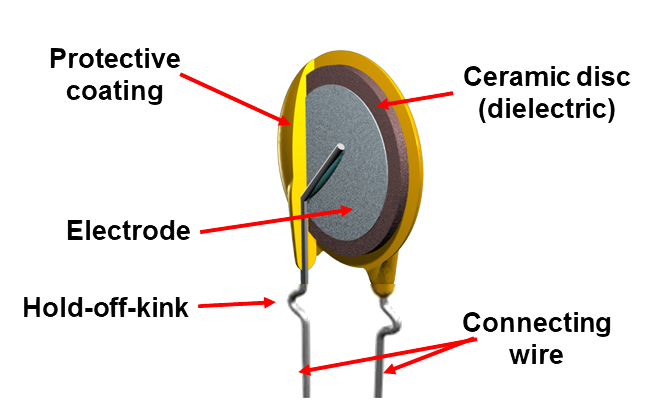
\includegraphics[keepaspectratio=true,scale=.5]{./figures/testImage.png}
    \centering
%    \cite{capSite_df_vs_temp}
    \caption{Dissipation Factor Plot}
    \label{dfPlot}
\end{figure}

The loss tangent can be seen in Figure: \ref{dfPlot}. The greater the angle, the more efficient the capacitor will be.

\subsection{Quality Factor}

\begin{equation}
\label{qual}
Q = \frac{1}{D}
\end{equation}

The Quality Factor, Q, of a capacitor is found by taking the reciprocal of the dissipation factor, Equation: \eqref{qual}. It is defined as the ratio of the energy stored to the energy dissipated per cycle.

\subsection{Insulation Resistance}

Every capacitor will have some DC leakage resistance associated with it. This measurement is attenuated by the insulation resistance of the capacitor. A high insulation resistance in a capacitor will increase its ability to store charge. This characteristic is especially important in sample and hold circuits.

\subsection{Dielectric Absorption}

Dielectric Absorption, DA, in a capacitor is a characteristic which describes the unit's ability to "regenerate" a charge after being shorted to ground for a brief time.

\begin{figure}
    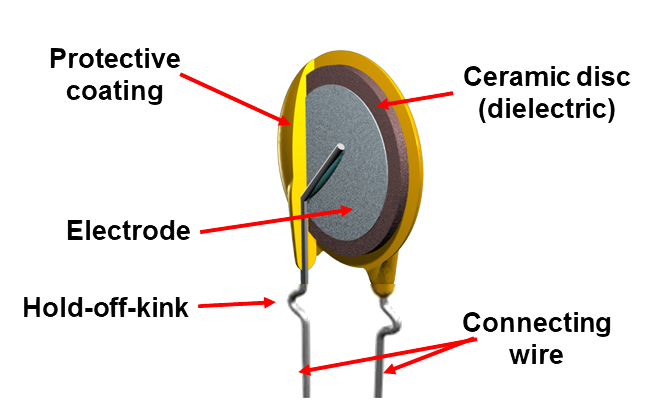
\includegraphics[keepaspectratio=true,scale=.5]{./figures/testImage.png}
    \centering
%    \cite{capSite_df_vs_temp}
    \caption{Dielectric Absorption}
    \label{daPlot}
\end{figure}

As seen in Figure: \ref{daPlot}, a capacitor can be modeled with multiple RC element, of a much greater time constant, in parallel with the bulk capacitance. When the main capacitor is shorted to ground, and then released, the other capacitors may not have released their energy. After several minutes, they can recharge the main capacitance to a significant portion of its original charge. This is why large valued electrolytic capacitors get shipped with a resistor across their terminals.

\subsection{Old}

This section will list and explain a large number of capacitor parameters. It will not deal with any analysis or measurement.

\begin {enumerate}
    \item Impedance
    \item Phase
    \item Capacitance
    \item Reactance
    \item Equivalent Series Resistance (ESR)
    \item Equivalent Series Inductance (ESI)
    \item Leakage current
    \item Dissipation factor
    \item Quality factor
    \item Dielectric absorption
    \item Loss Tangent
\end {enumerate}

\section {Measurement Circuitry}
This section describes the schematic design used to meet the goals set out in the Abstract (Section: \ref{sec:abstract}). The schematic can be found in the Appendix section: \ref{sec:schematic}.

\nocite{my_ieeePaper}

\subsection {DC Bias}
\label{sec:dcBias}

The DC bias control \hyperlink{sch:dcBias}{circuitry} controls a Stanford Research Supply SRS-PS350 power supply to generate the bias voltage for the circuit. Some of the models of this supply provide a serial input which can be used to set their output voltage. This scenario is preferred and the communications for it are handled through the RS232 transceiver found on Schematic Page: 3. Other models of this supply only provide an analog input option to control their output voltage. The specifications for this method are shown in Table: \ref{table:srsCtrl_table}. The control signal is generated by using the microcontroller to set the \gls{dac} output over a SPI bus. It is then buffered and clamped to under 1.5V. Since the SRS-PS350 has a gain of 500, this clamps its output to 750VDC. The circuit is only designed to operate at up to 500VDC, but this value is still within the specified ratings of the components in the signal path.

\begin{table}[ht!]
\centering
\begin{tabular}{| l | l | }
\hline
Input Scale      & 0 to +10V for 0 to 5kV                          \\ \hline
Input Impedance  & 1 M$\Omega$                                     \\ \hline
Accuracy         & $\pm 0.2\%$ of full scale                       \\ \hline
Update Rate      & 15 Hz                                           \\ \hline
Output Slew Rate & \textless 0.3s for 0 to full scale (full load)  \\ \hline
\end{tabular}
\caption{SRS-PS350 Analog Control Characteristics \cite{srsManual}\cite{srsCatalog}}
\label{table:srsCtrl_table}
\end{table}


The \gls{dac} has a 2.5V internal reference with a 14 bit resolution, giving the control signal an ideal resolution of $150\mu V$ and the SRS-PS350 an ideal output resolution of $76mV$. The update rate of this device is not important to this application because the \gls{dac} will be set infrequently and only when the system is not actively collecting data.

If different characteristics are needed, the SRS-PS350 can be exchanged for an alternate power supply, but the control logic may not be supported.


\subsection{Current Measurement}

Each of the tests utilize the low-side current measurement circuit. The AC measurement tests provide a known voltage across the DUT and then the current is used to construct the impedance. The discharge tests use the current measurement circuit to capture the current through the DUT over time as its energy drains. 

\subsection{Current Measurement}

Each of the tests utilize the low-side current measurement circuit. The AC measurement tests provide a known voltage across the DUT and then the current is used to construct the impedance. The discharge tests use the current measurement circuit to capture the current through the DUT over time as its energy drains. 

\input{tables/imeas}

The current measurement circuit utilizes a transimpedance amplifier designed from the reference circuit in \cite{steve_thesis}. It utilizes 3 switched, feedback stages to measure 9 decades of current (See Table: \ref{imeas_table}). The circuit creates a virtual ground at the negative terminal of the DUT and then uses one of the feedback paths to create a voltage for a digitizer. Using a low-side current measurement circuit is beneficial in this circumstance because it allows low voltage circuitry to condition and measure a signal without needing to see the high DC voltage on the positive terminal of the DUT. The output voltage is calculated by Equation: \eqref{trans}.

\begin{equation}
\label{trans}
Vo = I*R_f
\end{equation}

*Add transistor in increase the Op Amp's current drive capability.
*Change capacitors in feedback loop.
*Add Sallen-key filter to output
*Explain difference in two buffering stages


The output will be buffered and then filtered and digitized dependent of the specific test of interest.



The current measurement circuit utilizes a transimpedance amplifier designed from the reference circuit in \cite{steve_thesis}. It utilizes 3 switched, feedback stages to measure 9 decades of current (See Table: \ref{imeas_table}). The circuit creates a virtual ground at the negative terminal of the DUT and then uses one of the feedback paths to create a voltage for a digitizer. Using a low-side current measurement circuit is beneficial in this circumstance because it allows low voltage circuitry to condition and measure a signal without needing to see the high DC voltage on the positive terminal of the DUT. The output voltage is calculated by Equation: \eqref{trans}.

\begin{equation}
\label{trans}
Vo = I*R_f
\end{equation}

*Add transistor in increase the Op Amp's current drive capability.
*Change capacitors in feedback loop.
*Add Sallen-key filter to output
*Explain difference in two buffering stages


The output will be buffered and then filtered and digitized dependent of the specific test of interest.


\subsection{Charging Circuitry}
\label{sec:charging}

The \gls{dut} charging \hyperlink{sch:discharging}{circuitry} is meant to only be used to prepare the \gls{dut} for a test. The current is purposely limited in order to minimize the load on the SRS-PS350. The charging operation functions by enabling the high-current measurement and charging relays, and then slowly ramping the DC bias voltage until the \gls{dut} is fully charged.


\newpage
\section{Discharge Equations}
\label{app:disChargeEqs}
This section lists the discharge equations from Miller's electrochemical capacitor model \cite{electrochem_intro} seen in Figure: \ref{fig:superCap}.

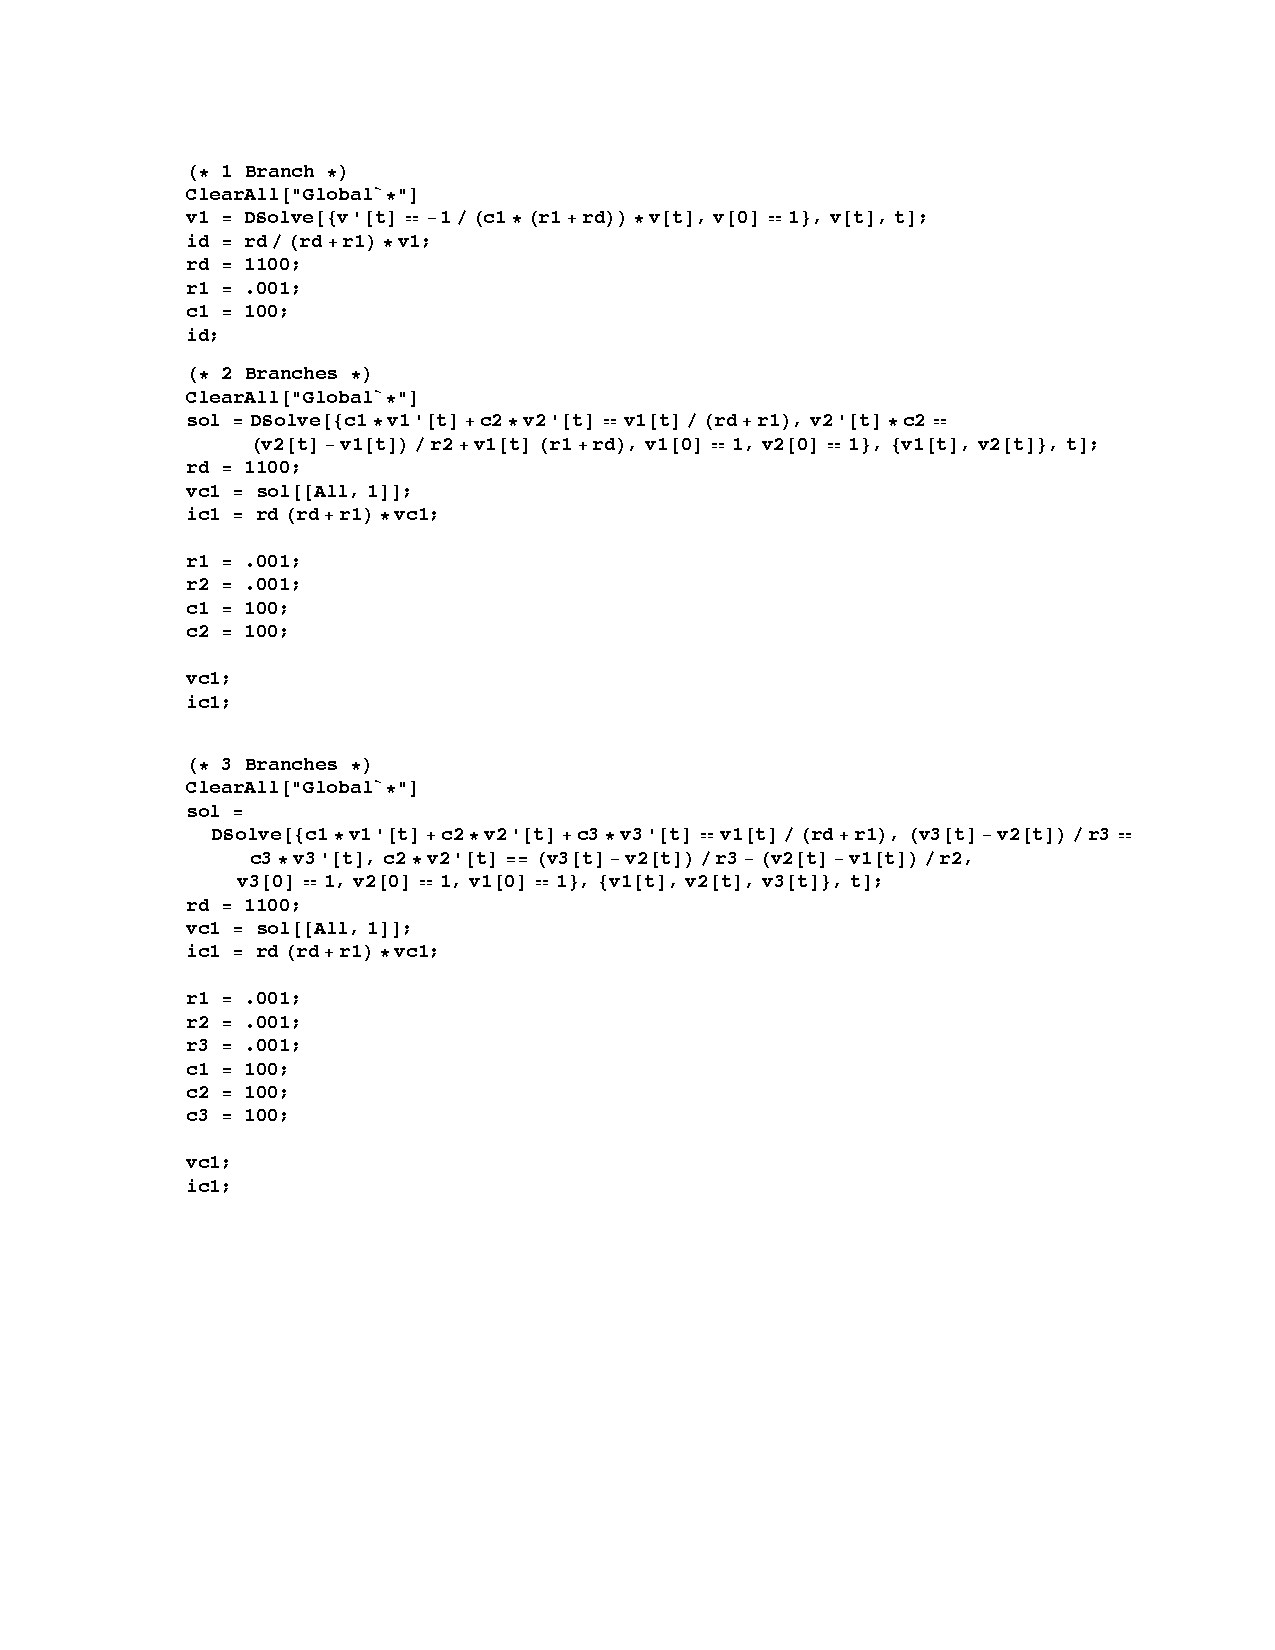
\includepdf[pages=-,offset=1.3in -1.3in,pagecommand={}]{scripts/discharge/discharge.pdf}

\subsection{Magnitude}

This setion describes the magnitude circutry shown on Schematic Page: 7. The circuit measures both the magnitude of the input sine wave and the magnitude of the resultant current waveform through the \gls{dut}. The design for this circuit is based off an Analog Device's app not for the AD8277 \cite{absCircuit}.

The function of this circuit is to perform a full-wave rectification operation on the input signal and then pass the output to be filtered and then sampled. The first difference amplifier is configured as a voltage follower. Since it is only powered from a single rail, it passes the positive half of the waveform and shunts the negative half to ground. The second difference amplifier operates in different modes, based upon the output of the first differential amplifier. During the negative going portions of the waveform, its positive terminal is held at ground, and it operates as a unity gain, inverting amplifier. This rectifies the input signal to the output. During the positive going portions of the waveform, positive input terminal is held at the value of the input terminal. This forces the second difference amplifier to act as a voltage follower. The resultant waveform is a full-wave recified version of the input signal. It is then bypassed with an output capacitor and fed into the \gls{adc} to calculate the value of the rms voltage.


\subsection{Phase}

This setion describes the phase circutry shown on Schematic Page: 7. The circuit measures both the phase of the input sine wave and the phase of the resultant current waveform through the \gls{dut}. It uses two, redundant phase measurement techniques.

The first technique utilizes the AD8302, a \gls{rf} phase detector, in a low frequency configuration as per AN-691 \cite{AD8302_AppNote}. The capacitors on the IC inputs tune the front end high pass filter cutoff to roughly 20Hz. The phase measurement is accomplished internally by a magnitude independent phase multiplier configuration. The output conisists of a 10mV per degree signal that is lowpassed at 2Hz to prevent aliasing. The filtered signal is then fed to the ADC for digitization.

The second technique is added for a low frequency comparison against the \gls{rf} phase detector. The comparator acts as a sine to square wave converter. The default configuration relies on the comparator's internal hysteresis, but provisions for wider thresholds are available if needed. The outputs of the two converters are fed into timer inputs on the microcontroller. The phase is then calculated by the \gls{mcu} by measuring the period of the signals and the time difference between their rising edges.


\subsection{Communications}

The communications \hyperlink{sch:com}{circuitry} is used to communicate to off-board processors.

\subsubsection{USB}
The \gls{usb} section is used to communicate with a PC for data logging and post processing. This circuitry centers around a FTDI FT232H serial to \gls{usb} chip. It allows seamless \gls{usb} communication to a PC's COM port with the \gls{mcu} only using a single UART port. This significantly lowers the complexity of the communication bus, as the \gls{mcu} is not responsible for running the \gls{usb} stack.

\subsubsection{RS-232}
The board also has two, bidirectional RS-232 ports. They are able to be used for general purposes, but will most often be used for communicating with a sine-wave generator and the DC Bias supply.



\section {Regression Analysis and Modeling}
\label{sec:regression}

Many designers have a need to simulate the response of the individual components in their systems for impulse and steady state inputs. When dealing with passive electronic components, the \gls{dut} is typically modeled as a combination of various resistors, capacitors, and inductors. The model chosen is often due to either the required accuracy or a specific characteristic of the \gls{dut} that needs to be modeled. When characterizing a new component, the complex frequency response is recorded and then fit to a model. In this section, a progression of regression techniques will be evaluated for their ability to fit the measured frequency response of a capacitor to a polynomial equation. Then the accuracy of various capacitor models will be explored in regards to the fit. All models will attempt to fit the capacitor impedance data shown Figure: \ref{fig:exCapData}. See Appendix: \ref{app:genModelingImages} for the code used to generate the images shown in this section.

% This figure was generated by ./scripts/modeling/plot_ExCapData.m
\begin{figure}[ht!]
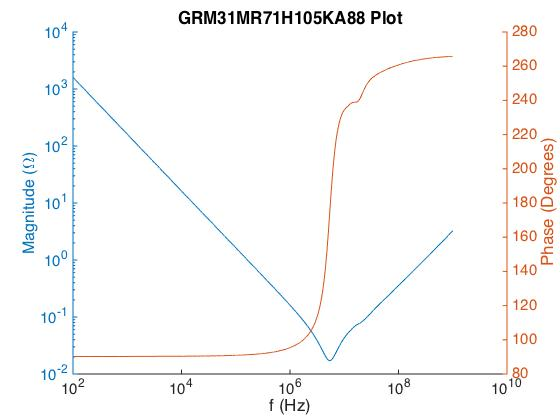
\includegraphics[keepaspectratio=true,width=6in]{./figures/modeling/exCapData.jpg}
\centering
\caption{GRM31MR71H105KA88 Capacitor Data}
\label{fig:exCapData}
\end{figure}


\subsection{Regression Analysis}
\label{sec:RegressionAnalysis}
\subsubsection{Basic LSE}
At its core, regression analysis is an optimization problem whose purpose is to fit the equation of a line to a data set. A commonly used regression analysis technique is called the \gls{lse}. It attempts to find a model which minimizes the squared error between an empirical set of data and itself.

The first step in applying an \gls{lse} is to choose the form of the equation that best represents the data. The equation of a line, Equation: \eqref{equ:ExLinEqu}, is chosen when only a simple linear fit is needed.
Then the squared error equation is generated, as in Equations: \eqref{equ:LSE_E2} \& \eqref{equ:LSE_E2b}.

\begin{equation}
\label{equ:ExLinEqu}
y = a_0 + a_1 x
\end{equation}

\begin{equation}
\label{equ:LSE_E2}
E^2 = \sum_{i=1}^{n} (y_i - y)^2
\end{equation}

\begin{equation}
\label{equ:LSE_E2b}
E^2 = \sum_{i=1}^{n} (y_i - (a_0 + a_1 x_i))^2
\end{equation}

In order to minimize the squared error over the data set, one needs to take the partial derivate of Equation: \eqref{equ:LSE_E2b} with respect to each of the unknown parameters, the coefficients, separately. While $a_0$ and $a_1$ will be constants in the final equation, they are treated as variables here until they are known. Conversely, all $x_i$ values are treated as constants. This results in Equations: \eqref{equ:LSE_PD1} \& \eqref{equ:LSE_PD2}.

\begin{align} 
    \frac{\partial E^2}{\partial a_0} &= 0 = \sum_{i=1}^{n} (-2y_i +2a_0 + 2a_1 x_i)           \label{equ:LSE_PD1} \\
    \frac{\partial E^2}{\partial a_1} &= 0 = \sum_{i=1}^{n} (-2y_i x_i +2a_0 x_i + 2a_1 x_i^2) \label{equ:LSE_PD2}
\end{align}

Up to this point most \gls{lse} methods analyze follow the same basic path. The rest of the steps will depend upon the complexity of the model and solution techniques. The following steps in the basic \gls{lse} use transformations and substitutions to solve for the unknown variables. In this case case, Equation: \eqref{equ:avgb} is used to remove the summation terms from the equation.

\begin{equation}
    \label{equ:avgb} 
    \sum_{i=1}^{n} y_i  = \bar{y}n
\end{equation}

This results in Equations: \eqref{equ:LSE_sol} \& \eqref{equ:LSE_solb} with solutions shown in Equations: \eqref{equ:LSE_solc} \& \eqref{equ:LSE_sold}. The empirical data is then used to find the values of $a_0$ and $a_1$. At this point, the best fit line can be used to estimate new points on the plot or to compare against other data sets (Figure: \ref{fig:basicLSE}).

\begin{figure}[ht!]
\ifisPPT
\noindent\makebox[\textwidth]{\includegraphics[keepaspectratio=true,width=\paperwidth]{../figures/regression/basicLSE.jpg}}
\else
\includegraphics[keepaspectratio=true,width=6in]{./figures/regression/basicLSE.jpg}
\fi
\centering
\caption{Basic LSE}
\label{fig:basicLSE}
\end{figure}



\begin{equation}
    \label{equ:LSE_sol}
    0 = \bar{y} - (a_0 + 2a_1 \bar{x})
\end{equation}

\begin{equation}
    \label{equ:LSE_solb}
    0 = \bar{xy} - (a_0 \bar{x} + 2a_1 \bar{x^2})
\end{equation}

\begin{equation}
    \label{equ:LSE_solc}
    a_0 = \bar{y} - a_1 \bar{x}
\end{equation}

\begin{equation}
    \label{equ:LSE_sold}
    a_1 = \frac{\bar{xy} - \bar{x}\bar{y}}{\bar{x^2} - \bar{x}^2}
\end{equation}

\subsubsection{Levy's Technique - Complex Curve Fitting}
While the basic \gls{lse} technique is sufficient for many circumstances, it is not directly applicable in situations where one needs to fit a model to a complex line, such as a transfer function. Levy \cite{levy} shows an extension of the simple \gls{lse} example that is valid for a generic polynomial transfer function. This method is important because it not only allows for a complex-valued transfer function, but it also prevents the necessity of rederiving the system of equations for each new model. 

\begin{equation}
    \label{equ:levy_Gs}
    G(s) = \frac{A_0 + A_1 s + A_2 s^2 + ... + A_n s^n}{B_0 + B_1 s + B_2 s^2 + ... + B_m s^m}
    ~\cite{levy}[Eq.~3]
\end{equation}

Using Equation: \eqref{equ:levy_Gs} as the generic model, Levy shows that you can use Equations: \eqref{equ:Levy_L}, \eqref{equ:Levy_S}, \eqref{equ:Levy_T}, \& \eqref{equ:Levy_U} to simplify the series of partial derivatives into a single matrix multiplication equation shown in \eqref{equ:Levy_Ans}, \eqref{equ:Levy_M}, \eqref{equ:Levy_N}, \& \eqref{equ:Levy_C}.

\begin{equation}
    \label{equ:Levy_L}
    \lambda _h = \sum_{k=0}^{m} \omega _k ^h
    ~\cite{levy}[Eq.~15]
\end{equation}

\begin{equation}
    \label{equ:Levy_S}
    S_h = \sum_{k=0}^{m} \omega _k ^h R_k
    ~\cite{levy}[Eq.~16]
\end{equation}

\begin{equation}
    \label{equ:Levy_T}
    T_h = \sum_{k=0}^{m} \omega _k ^h I_k
    ~\cite{levy}[Eq.~17]
\end{equation}

\begin{equation}
    \label{equ:Levy_U}
    U_h = \sum_{k=0}^{m} \omega _k ^h (R_k ^2 + I_k ^2)
    ~\cite{levy}[Eq.~18]
\end{equation}

\begin{equation}
    \label{equ:Levy_Ans}
    MN = C
    ~\cite{levy}[Eq.~20]
\end{equation}

\setcounter{MaxMatrixCols}{12} % Allows each row of M to fit on one line
\begin{equation}
\label{equ:Levy_M}
M = 
\begin{bmatrix}
\lambda _0 & 0          & -\lambda _2 &  0           & \lambda _4  & \cdots &  T_1    & S_2    & -T_3   & -S_4   &  T_5    & \cdots \\
0          & \lambda _2 & 0           & -\lambda _4  & 0           & \cdots & -S_2    & T_3    &  S_4   & -T_5   & -S_6    & \cdots \\
\lambda _2 & 0          & -\lambda _4 &  0           & \lambda _6  & \cdots &  T_3    & S_4    & -T_5   & -S_6   &  T_7    & \cdots \\
0          & \lambda _4 & 0           & -\lambda _6  & 0           & \cdots & -S_4    & T_5    &  S_6   & -T_7   & -S_8    & \cdots \\

\vdots     & \vdots     &  \vdots     & \vdots       & \vdots      &        &  \vdots & \vdots & \vdots & \vdots &  \vdots &        \\ 
T_1        & -S_2       & -T_3        &  S_4         & T_5         & \cdots &  U_2    & 0      & -U_4   &  0     &  U_6    & \cdots \\
S_2        &  T_3       & -S_4        & -T_5         & S_6         & \cdots &  0      & U_4    &  0     & -U_6   &  0      & \cdots \\
T_3        & -S_4       & -T_5        &  S_6         & T_7         & \cdots &  U_4    & 0      & -U_6   &  0     &  U_8    & \cdots \\
\vdots     & \vdots     &  \vdots     & \vdots       & \vdots      & \vdots &  \vdots & \vdots & \vdots & \vdots &  \vdots &        \\ 
\end{bmatrix}
~\cite{levy}[Eq.~21a]
\end{equation}

\begin{multicols}{2}
    \begin{equation}
        \label{equ:Levy_N}
        N = 
        \begin{bmatrix}
            A_0 \\
            A_1 \\
            A_2 \\
            A_3 \\
            \vdots \\
            B_1 \\
            B_2 \\
            B_3 \\
            \vdots
        \end{bmatrix}
        ~\cite{levy}[Eq.~21b]
    \end{equation}

    \begin{equation}
        \label{equ:Levy_C}
        C = 
        \begin{bmatrix}
            S_0 \\
            T_1 \\
            S_2 \\
            T_3 \\
            \vdots \\
            0   \\
            U_2 \\
            0   \\
            \vdots
        \end{bmatrix}
        ~\cite{levy}[Eq.~21c]
    \end{equation}
\end{multicols}

Levy's technique works well for applications where there is a small dynamic frequency range and a small number of coefficients, but there a several problems with it.
The first problem is that for models with a wide bandwidth, the solution to Equation: \eqref{equ:Levy_Ans}, involves an ill-conditioned matrix. This means that the solution to the system of equations will experience precision errors.
The second problem is that this technique is heavily biased by high frequency data. As can be seen in Figure: \ref{fig:levy}, applying Levy's technique with a $3^{rd}$ order model provides a unusable fit to the empirical data.

% Run /scripts/regression/run_levy_iter.m with NumDeg = 3, DenDeg = 3, and iterations = 1.
\begin{figure}[ht!]
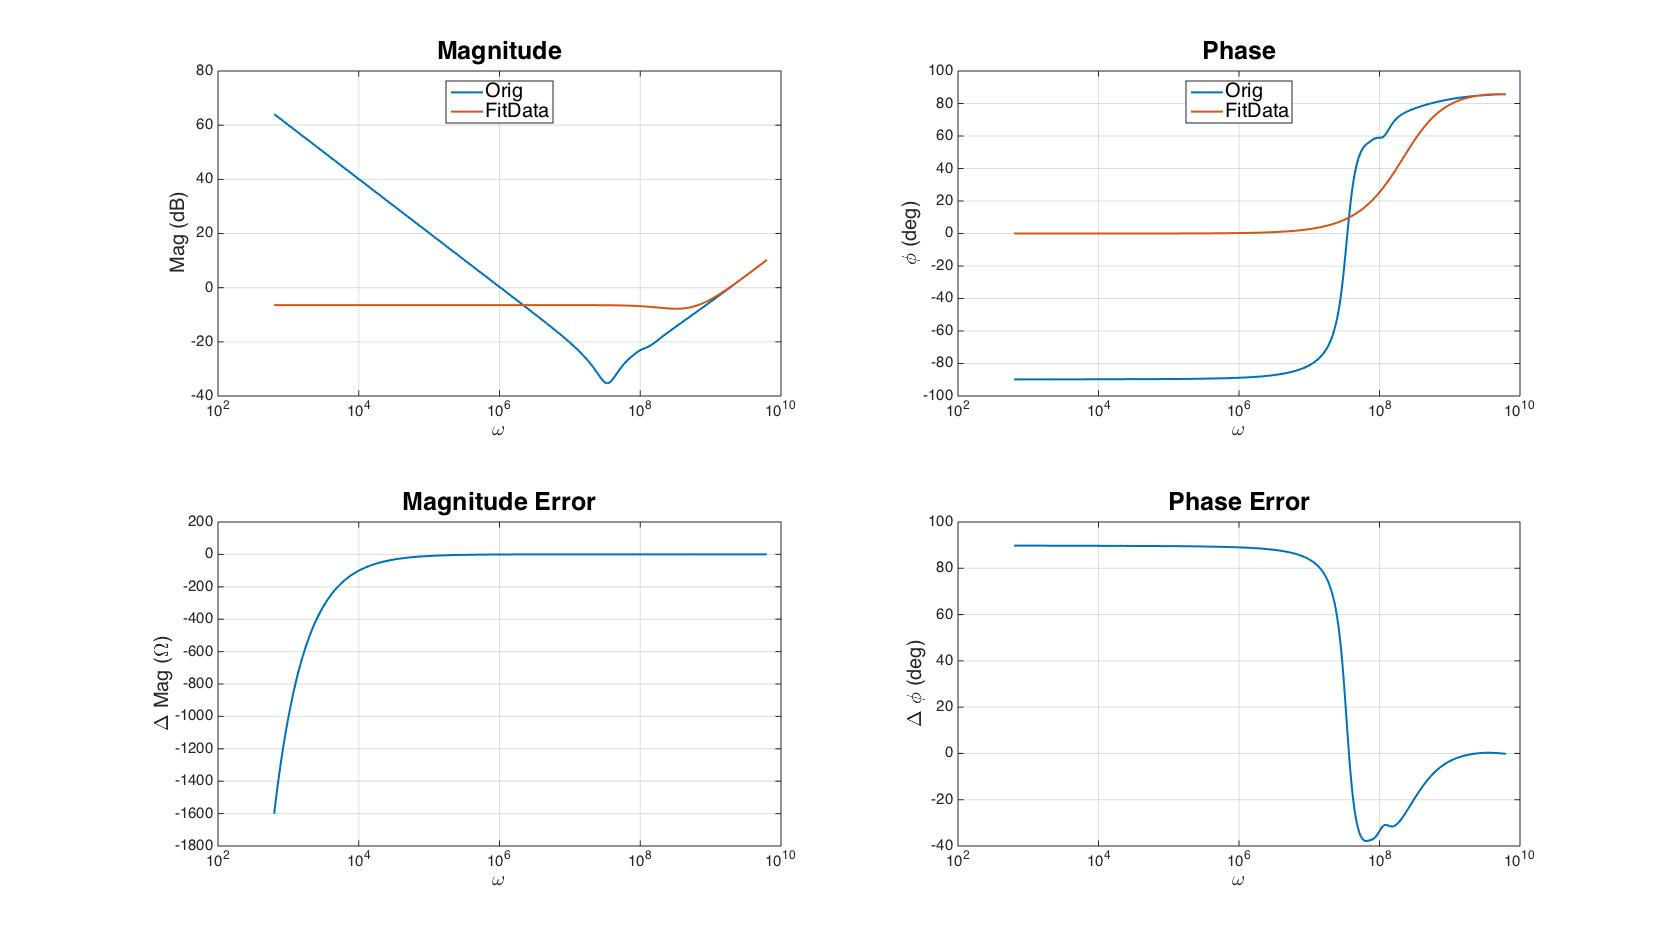
\includegraphics[keepaspectratio=true,width=6in]{./figures/regression/levy.jpg}
\centering
\caption{Levy's Technique}
\label{fig:levy}
\end{figure}



\subsubsection{Weighted LSE}
\label{sec:weightedLSE}
One improvement that can be made upon Levy's method is to iterate with a frequency dependent weighting function until the error term is minimized \cite{levy_iter}. By multiplying Levy's error function by the weighting term in Equation: \eqref{equ:iter_Weight}, we get Equation: \eqref{equ:iter_Err}, which can be used to obtain a new system of equations.
The $L$ subscript stands for the current iteration, while $L-1$ stands for the previous iteration.

\begin{equation}
    \label{equ:iter_Weight}
    W_{kL} = \frac{1}{|Q(jw_k)_{L-1}|^2}
    ~\cite{levy_iter}
\end{equation}

\begin{equation}
    \label{equ:iter_Err}
    E = \sum_{k=1}^{n} |\epsilon _k ^{'}|^2W_{kL}
    ~\cite{levy_iter}[Eq.~7]
\end{equation}

Equations \eqref{equ:Levy_Ans}, \eqref{equ:Levy_M}, \eqref{equ:Levy_N}, \& \eqref{equ:Levy_C} are the same, with Equations \eqref{equ:Levy_L}, \eqref{equ:Levy_S}, \eqref{equ:Levy_T}, \& \eqref{equ:Levy_U} being replaced with Equations: \eqref{equ:Iter_L}, \eqref{equ:Iter_S}, \eqref{equ:Iter_T}, \& \eqref{equ:Iter_U}.

\begin{equation}
    \label{equ:Iter_L}
    \lambda _h = \sum_{k=0}^{m} \omega _k ^hW_{kL}
    ~\cite{levy_iter}[Eq.~9]
\end{equation}

\begin{equation}
    \label{equ:Iter_S}
    S_h = \sum_{k=0}^{m} \omega _k ^h R_kW_{kL}
    ~\cite{levy_iter}[Eq.~10]
\end{equation}

\begin{equation}
    \label{equ:Iter_T}
    T_h = \sum_{k=0}^{m} \omega _k ^h I_kW_{kL}
    ~\cite{levy_iter}[Eq.~11]
\end{equation}

\begin{equation}
    \label{equ:Iter_U}
    U_h = \sum_{k=0}^{m} \omega _k ^h (R_k ^2 + I_k ^2)W_{kL}
    ~\cite{levy_iter}[Eq.~12]
\end{equation}

Dependent upon the initial conditions and the model order, this particular method is not guaranteed to converge. Figure: \ref{fig:levyIter_Err1} was generated with an initial condition of $Q(jw_k) == 1$ and a model order of 7. It shows that, for this data set, the squared error of the magnitude and phase do not converge after a particular number of iterations. Furthermore, they do not reach their minimums at the same iteration. In order to select the desired iteration, the magnitude and phase squared plots are normalized as in Equation: \eqref{equ:ErrMin}. The index of the minimum of Figure: \ref{fig:levyIter_Err1} is selected as the best fit.

\begin{equation}
\label{equ:ErrMin}
n = min(\frac{E_{Mag}}{max(E_{Mag})} + \frac{E_{pha}}{max(E_{Pha})})
\end{equation}

\begin{figure}[ht!]
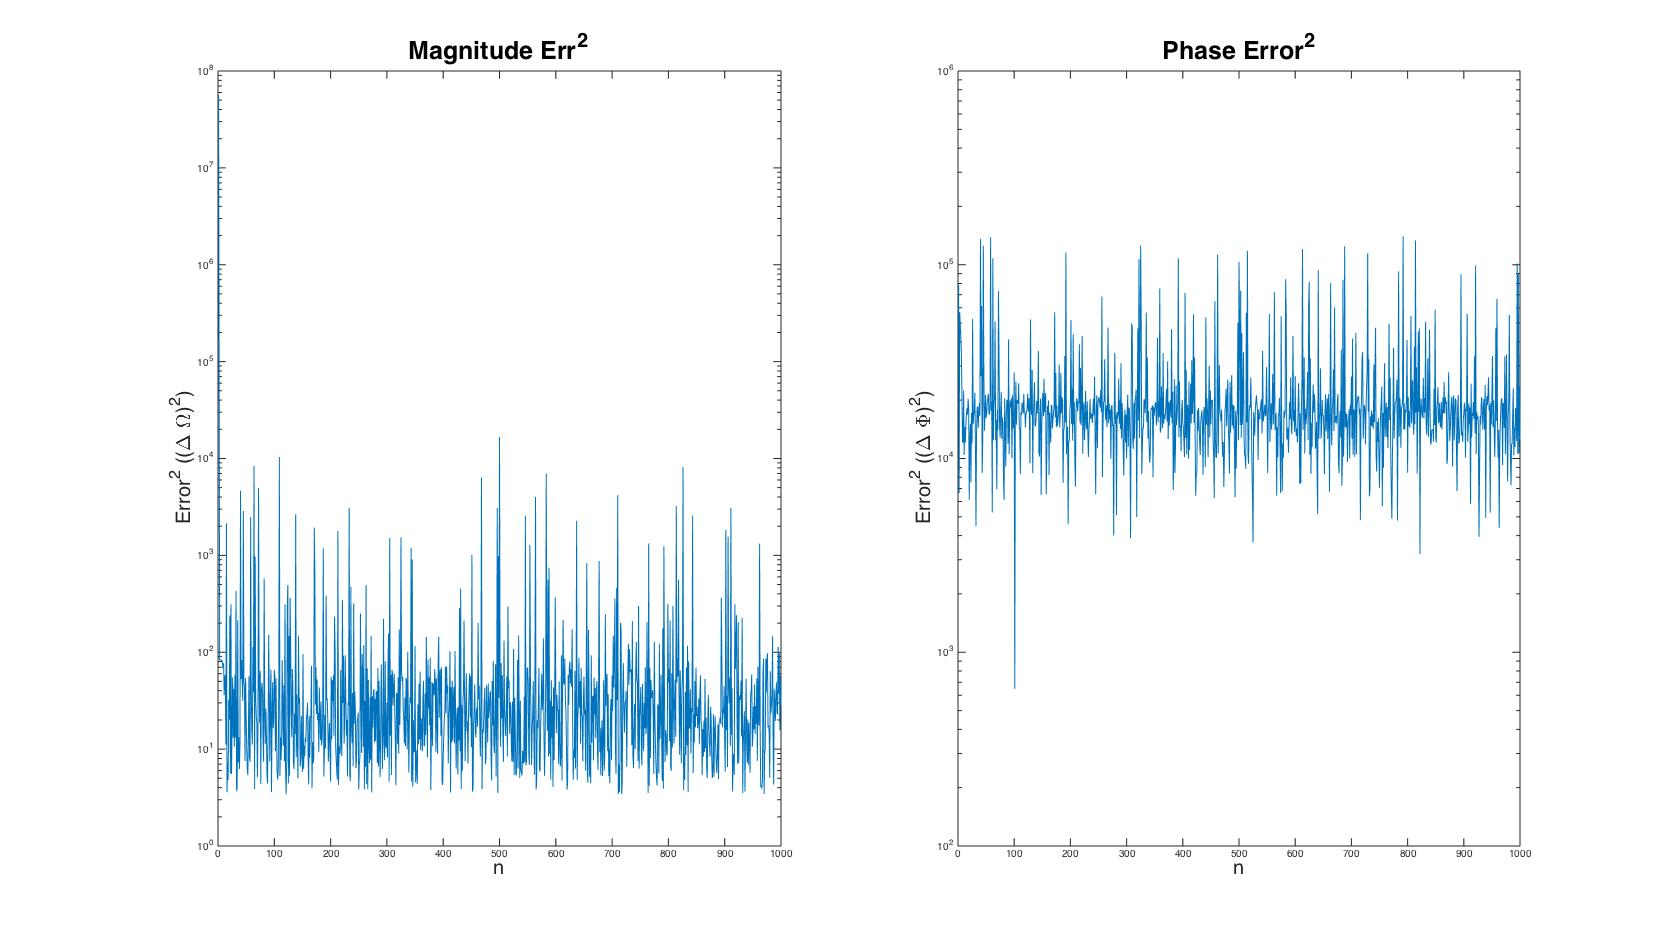
\includegraphics[keepaspectratio=true,width=6in]{./figures/modeling/levyIter_Err1.jpg}
\centering
\caption{LSE + Iteration -- Magnitude and Phase Error}
\label{fig:levyIter_Err1}
\end{figure}

% Run ./scripts/regression/run_levy_iter.m with numDeg = 7, denDeg = 7, and iterations = 100 to obtain this image.
\begin{figure}[ht!]
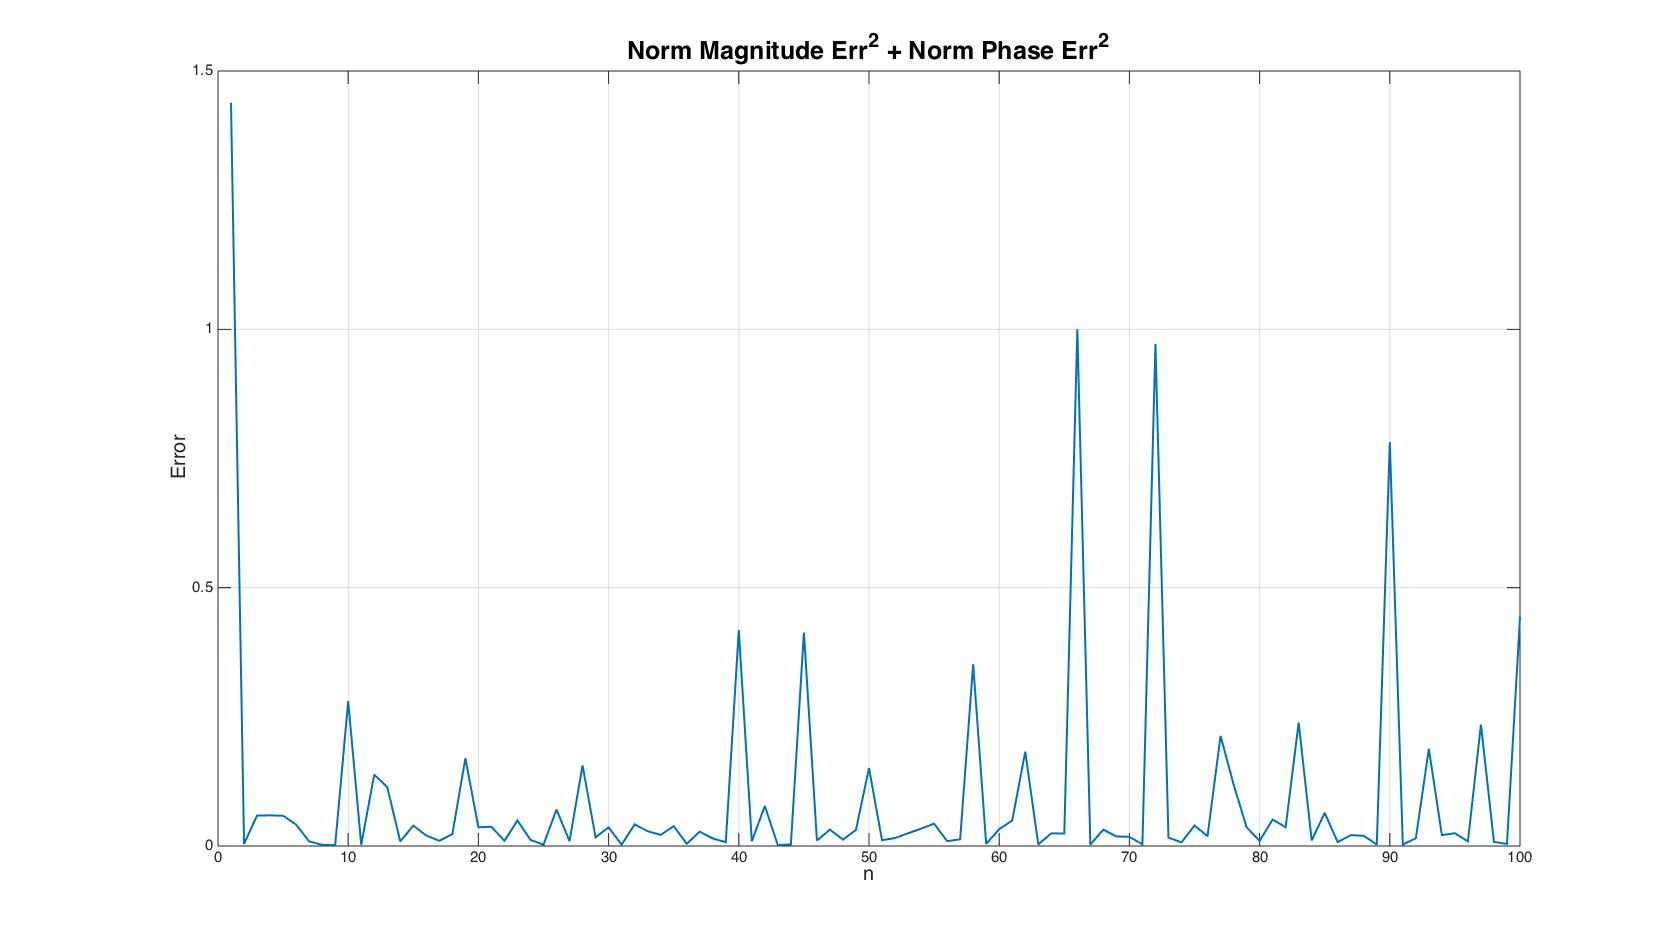
\includegraphics[keepaspectratio=true,width=6in]{./figures/regression/levyIter_Err2.jpg}
\centering
\caption{LSE + Iteration -- Combined Error}
\label{fig:levyIter_Err2}
\end{figure}



Figure: \ref{fig:levyIter} shows that this method can result in a much improved result over the Levy's original method, as seen in Figure: \ref{fig:levy}.

\begin{figure}
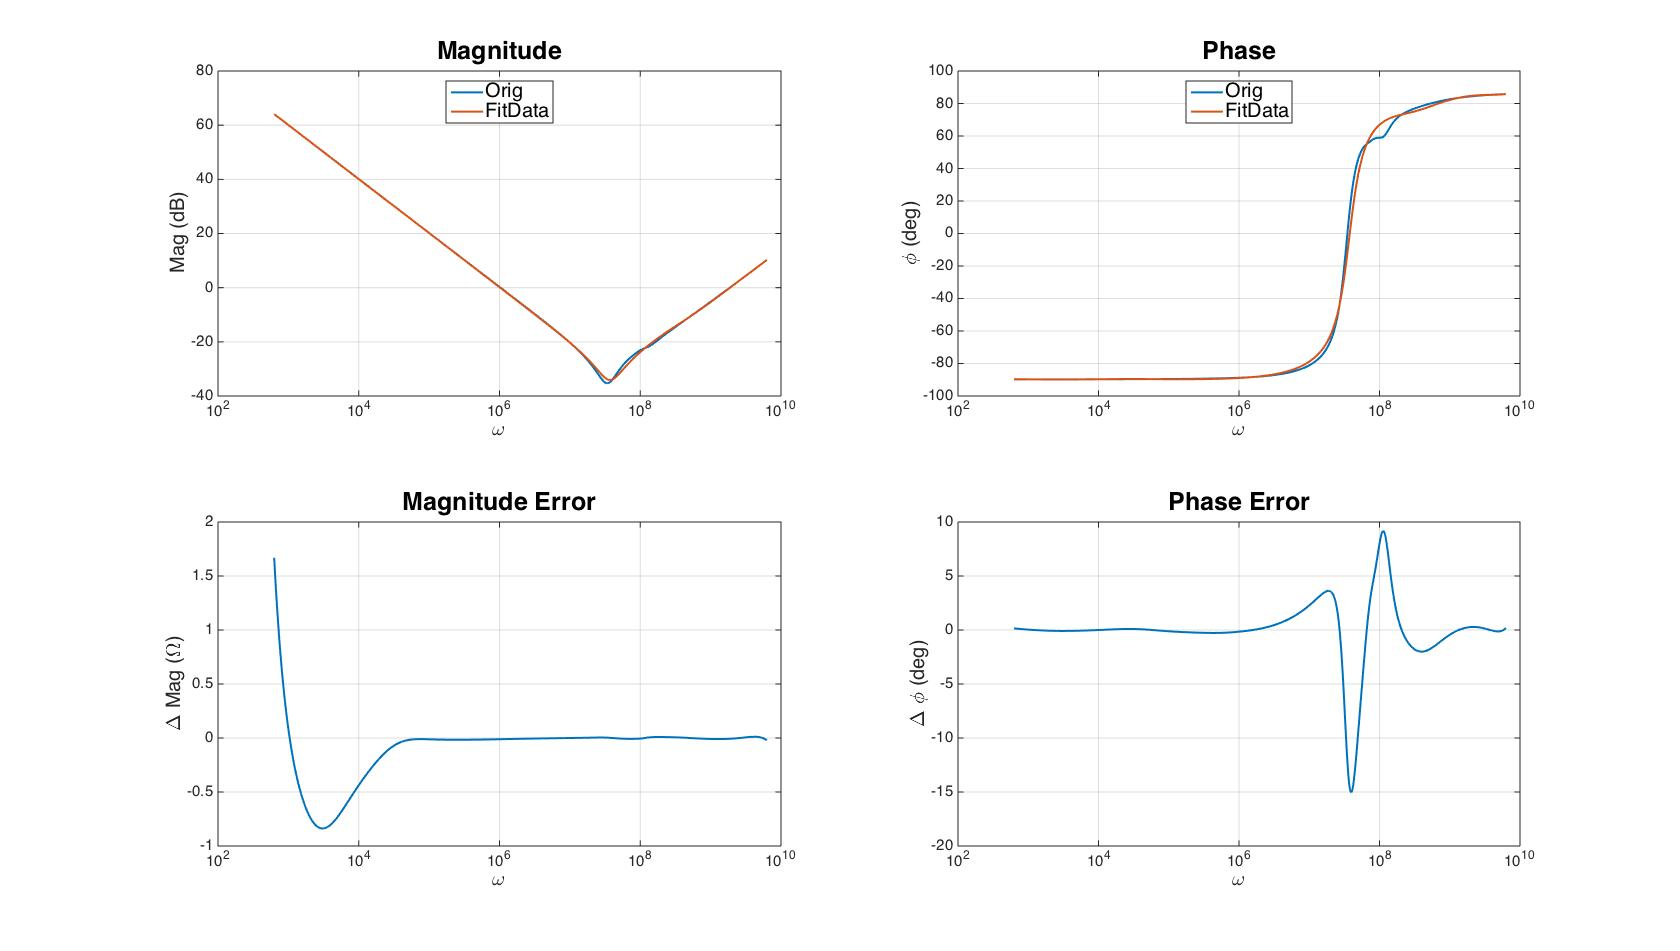
\includegraphics[keepaspectratio=true,width=6in]{./figures/modeling/levyIter.jpg}
\centering
\caption{LSE + Iteration}
\label{fig:levyIter}
\end{figure}


\subsection{Modeling}
This section will investigate several of the most common capacitor models. It will show how to fit them to a data set with Levy's method described in Section: \ref{sec:RegressionAnalysis}, and will describe their effectiveness and limitations in doing so.

\subsubsection{6 Term Model}
\begin{figure}[ht!]
\ifisPPT
\noindent\makebox[\textwidth]{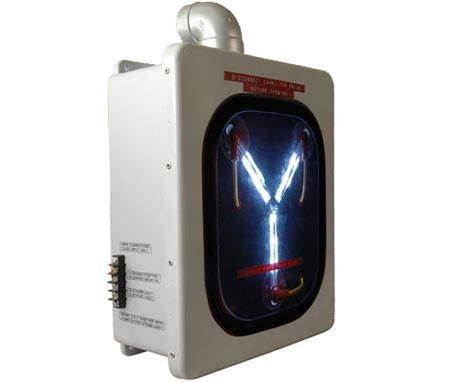
\includegraphics[keepaspectratio=true,width=\paperwidth]{../figures/regression/fullModel.jpg}}
\else
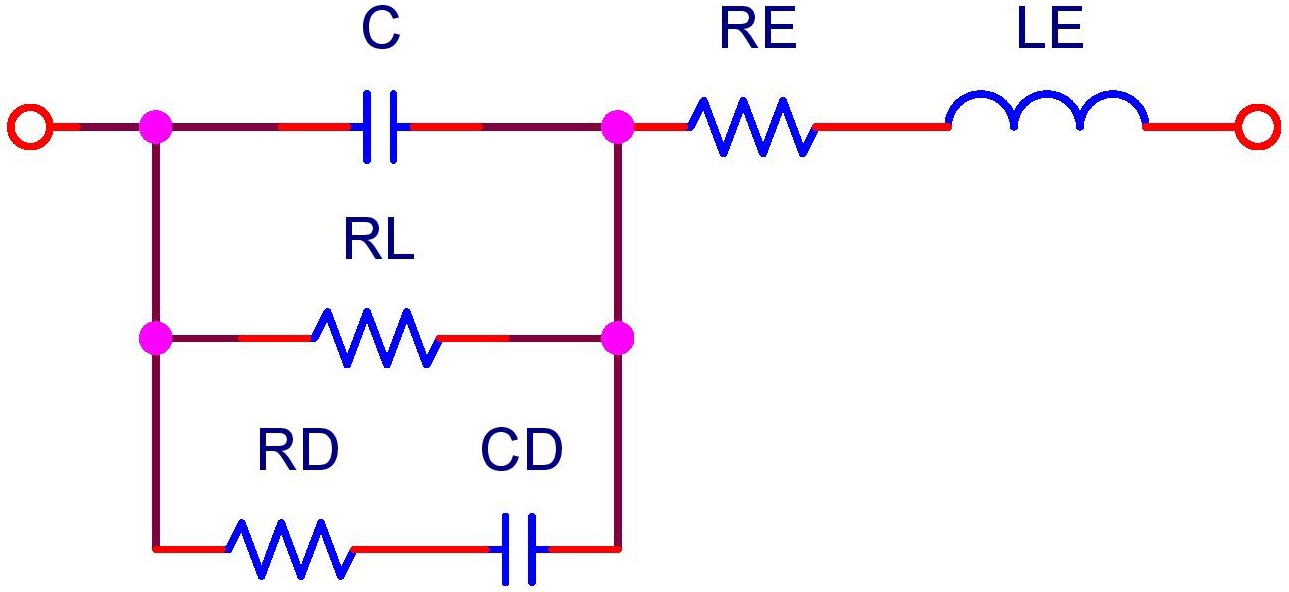
\includegraphics[keepaspectratio=true,width=2in]{./figures/regression/fullModel.jpg}
\fi
\centering
\caption{6 Term Model}
\label{fig:fullModel}
\end{figure}


The model shown in Figure: \ref{fig:fullModel} shows several of the most important parameters for a capacitor. It's impedance, shown in Equation: \eqref{equ:fullModelImpedance}, and generalized in Equation: \eqref{equ:fullModelPoly} can be used as the basis for a regression analysis.

\begin{equation}
    \begin{split}
        \label{equ:fullModelImpedance}
        \bar{Z}(s) = \frac{(R_E + R_L) + (L_E + C_DR_DR_E + C_DR_DR_L + CR_ER_L + C_DR_ER_L)s}{1 + (C_DR_D + CR_L + C_DR_L)s + CC_DR_DR_Ls^2} \\ 
        + \frac{(C_DL_ER_D + CL_ER_L + C_DL_ER_L + CC_DR_DR_ER_L)s^2 + CC_DL_ER_DR_Ls^3}{1 + (C_DR_D + CR_L + C_DR_L)s + CC_DR_DR_Ls^2}
    \end{split}
\end{equation}

\begin{equation}
    \label{equ:fullModelPoly}
    \bar{Z}(s) = \frac{a_0 + a_1s + a_2s^2 + a_3s^3}{b_0 + b_1s + b_2s^2}
\end{equation}


For this model, Equations: \eqref{equ:Levy_M}, \eqref{equ:Levy_N}, \& \eqref{equ:Levy_C} simplify down to Equations: \eqref{equ:fullModel_M}, \eqref{equ:fullModel_N}, \& \eqref{equ:fullModel_C}.

\begin{equation}
    \label{equ:fullModel_M}
    M = 
    \begin{bmatrix}
        \lambda _0 & 0          & -\lambda _2 & 0           &  T_1    & S_2 \\
        0          & \lambda _2 & 0           & -\lambda _4 & -S_2    & T_3 \\
        \lambda _2 & 0          & -\lambda _4 & 0           &  T_3    & S_4 \\
        0          & \lambda _4 & 0           & -\lambda _6 & -S_4    & T_5 \\
        T_1        & -S_2       & -T_3        &  S_4        &  U_2    & 0   \\
        S_2        &  T_3       & -S_4        & -T_5        &  0      & U_4
    \end{bmatrix}
\end{equation}

\begin{multicols}{2}
    \begin{equation}
        \label{equ:fullModel_N}
        N = 
        \begin{bmatrix}
            A_0 \\
            A_1 \\
            A_2 \\
            A_3 \\
            B_1 \\
            B_2
        \end{bmatrix}
    \end{equation}

    \begin{equation}
        \label{equ:fullModel_C}
        C = 
        \begin{bmatrix}
            S_0 \\
            T_1 \\
            S_2 \\
            T_3 \\
            0   \\
            U_2
        \end{bmatrix}
    \end{equation}
\end{multicols}

Using this model, the regression analysis method described in Section: \ref{sec:weightedLSE} generates the output seen in Figure: \ref{fig:fullModel_BadOutput}. The fit tracks the original data well, except at low frequencies and near resonance.

\begin{figure}[ht!]
\ifisPPT
\noindent\makebox[\textwidth]{\includegraphics[keepaspectratio=true,width=\paperwidth]{../figures/regression/fullModel_BadOutput.jpg}}
\else
\includegraphics[keepaspectratio=true,width=6in]{./figures/regression/fullModel_BadOutput.jpg}
\fi
\centering
\caption{6 Term Model: Bad Initilization}
\label{fig:fullModel_BadOutput}
\end{figure}


Substituting the polynomial coefficients seen in Equation: \eqref{equ:fullModel_BadOutputCoeff} into Equations: \eqref{equ:fullModel_CoeffEq_a0}-\eqref{equ:fullModel_CoeffEq_b2}, returns the model parameter values as seen in Equation: \eqref{equ:fullModel_BadOutputParams}.

\begin{align}
     a_0 &= R_E + R_L                                         \label{equ:fullModel_CoeffEq_a0} \\
     a_1 &= L_E + C_DR_DR_E + C_DR_DR_L + CR_ER_L + C_DR_ER_L \label{equ:fullModel_CoeffEq_a1} \\
     a_2 &= C_DL_ER_D + CL_ER_L + C_DL_ER_L + CC_DR_DR_ER_L   \label{equ:fullModel_CoeffEq_a2} \\
     a_3 &= CC_DL_ER_DR_L                                     \label{equ:fullModel_CoeffEq_a3} \\
     b_0 &= 1                                                 \label{equ:fullModel_CoeffEq_b0} \\
     b_1 &= C_DR_D + CR_L + C_DR_L                            \label{equ:fullModel_CoeffEq_b1} \\
     b_2 &= CC_DR_DR_L                                        \label{equ:fullModel_CoeffEq_b2}
\end{align}

Even though the polynomial coefficients gave an acceptable fit to the data, it resulted in unacceptable circuit parameters. Since $C$ and $R_D$ are negative, this model is not physically realizable.

\begin{multicols}{2}
    \begin{equation}
        \label{equ:fullModel_BadOutputCoeff}
        \begin{split}
             a_0 &= 5.9991E^{+03} \\
             a_1 &= 1.7934E^{-04} \\
             a_2 &= 3.3158E^{-12} \\
             a_3 &= 6.8295E^{-22} \\
             b_0 &= 1.0000        \\
             b_1 &= 5.9057E^{-03} \\
             b_2 &= 1.4067E^{-12}
        \end{split}
    \end{equation}

    \begin{equation}
        \label{equ:fullModel_BadOutputParams}
        \begin{split}
            C &= -8.2563E^{-10} \\
            R_E &=  3.1886E^{-01} \\
            L_E &=  4.8551E^{-10} \\
            R_L &=  4.8551E^{-10} \\
            C_D &=  9.8536E^{-07} \\
            R_D &= -2.8824E^{-01}
        \end{split}
    \end{equation}
\end{multicols}

This problem stems from the author's \cite{levy_iter} suggestion that the initial guess for $Q(jw_k) == 1$. While an initial guess is required to calculate the weighting function during the first iteration, this particular choice causes the problem seen in Equations: \eqref{equ:fullModel_BadInputCoeff} \& \eqref{equ:fullModel_BadInputParams} for this application. They show that this initial condition does not start with rational solution for the circuit parameters.

\begin{multicols}{2}
    \mbox{}\vfill
    \begin{equation}
        \label{equ:fullModel_BadInputCoeff}
        \begin{split}
            &a_0 = 1 \\
            &a_1 = 1 \\
            &a_2 = 1 \\
            &a_3 = 1 \\
            &b_0 = 1 \\
            &b_1 = 0 \\
            &b_2 = 0
        \end{split}
    \end{equation}

    \mbox{}\vfill
    \columnbreak

    \mbox{}\vfill
    \begin{equation}
        \label{equ:fullModel_BadInputParams}
        \begin{split}
             C   &= INF \\
             R_E &= INF \\
             L_E &= INF \\
             R_L &= IND \\
             C_D &= IND \\
             R_D &= IND \\
        \end{split}
    \end{equation}
    \mbox{}\vfill
\end{multicols}

Starting instead with the rational set of circuit parameters seen in Equation: \eqref{equ:fullModel_GoodInputParams}, the starting coefficients are as seen in Equation: \eqref{equ:fullModel_GoodInputCoeff}.

\begin{multicols}{2}
    \mbox{}\vfill
    \begin{equation}
        \label{equ:fullModel_GoodInputCoeff}
        \begin{split}
             a_0 &= 2 \\
             a_1 &= 5 \\
             a_2 &= 4 \\
             a_3 &= 1 \\
             b_0 &= 1 \\
             b_1 &= 3 \\
             b_2 &= 1
        \end{split}
    \end{equation}

    \mbox{}\vfill
    \columnbreak

    \mbox{}\vfill
    \begin{equation}
        \label{equ:fullModel_GoodInputParams}
        \begin{split}
             C   &= 1 \\
             R_E &= 1 \\
             L_E &= 1 \\
             R_L &= 1 \\
             C_D &= 1 \\
             R_D &= 1 \\
        \end{split}
    \end{equation}
    \mbox{}\vfill
\end{multicols}

\begin{figure}[ht!]
\ifisPPT
\noindent\makebox[\textwidth]{\includegraphics[keepaspectratio=true,width=\paperwidth]{../figures/regression/fullModel_GoodOutput.jpg}}
\else
\includegraphics[keepaspectratio=true,width=6in]{./figures/regression/fullModel_GoodOutput.jpg}
\fi
\centering
\caption{6 Term Model: Good Initilization}
\label{fig:fullModel_GoodOutput}
\end{figure}


Figure: \ref{fig:fullModel_GoodOutput} shows a good fit across the frequency spectrum for both magnitude and phase. The model does deviate at resonance, but that is not surprising, as the number of parameters in the model is fairly low when compared with the model used to generate the data.


\section {Conclusion}
\label{sec:conclusion}

\ifisPPT
\begin{frame}
    \frametitle{Conclusion}

Circuit Capabilities:
\begin{itemize}
    \item Discharge Curve
    \item Impedance
\end{itemize}

Measurement Range:
\begin{itemize}
    \item DC bias range 0$\rightarrow$500V.
    \item Frequency Range of 100Hz$\rightarrow$40kHz.
\end{itemize}

Regression Accuracy:
\begin{itemize}
    \item Accurrate outside of resonance.
    \item $2 \Omega$ and $2^{\circ}$.
    \item $<5\%$.
\end{itemize}
\end{frame}
\else
In conclusion, the circuitry and regression analysis developed in this thesis shows a promising ability to accurately model capacitors. The method shown provides the ability to model a capacitor over a 0 $\rightarrow$ 500VDC bias and a 100Hz $\rightarrow$ 40kHz range. The regression analysis provides a means to compare new capacitors with unknown characteristics. The accuracy of the model is mostly determined by the number of parameters and typically has the greatest relative error near resonance. Outside of resonance and low frequencies, the accuracy of the fit stays within $2 \Omega$ and $2^{\circ}$. The relative error, outside of a single peak in the phase plot, stays well below $5\%$. This method provides a good estimate of titanium capacitor parameters, which are best suited for power applications  at low frequencies.
\fi


\section {Future Work}
\label{sec:futureWork}

\newcommand{\futWorkCmd}
{
\begin{itemize}
    \item Build the circuit and validate against the stated capabilities and accuracy.
    \item Increase the available frequency range for the measurement circuitry.
    \item Add additional fail-safe protection to the circuit.
    \item Update the regression technique for better accuracy\ifisPPT \else~(See Section: \ref{app:adtl_regression})\fi.
    \item Evaluate the accuracy of the six term model\ifisPPT \else described in Section: \ref{sec:regression} with actual data\fi.
\end{itemize}
}

\ifisPPT
\begin{frame}
    \frametitle{Future Work}
    \futWorkCmd
\end{frame}
\else
This section will describe the future work that needs to be accomplished in order to complete and further the stated goals of this thesis. It will focus on the practical circuitry implementation and other aspects needed to make it a viable tool.

\futWorkCmd
\fi


\appendix{}
\appendixheaderon

\section{Schematic}
\label{app:schematic}
This section shows the schematic described in Section: \ref{sec:measCirc}.
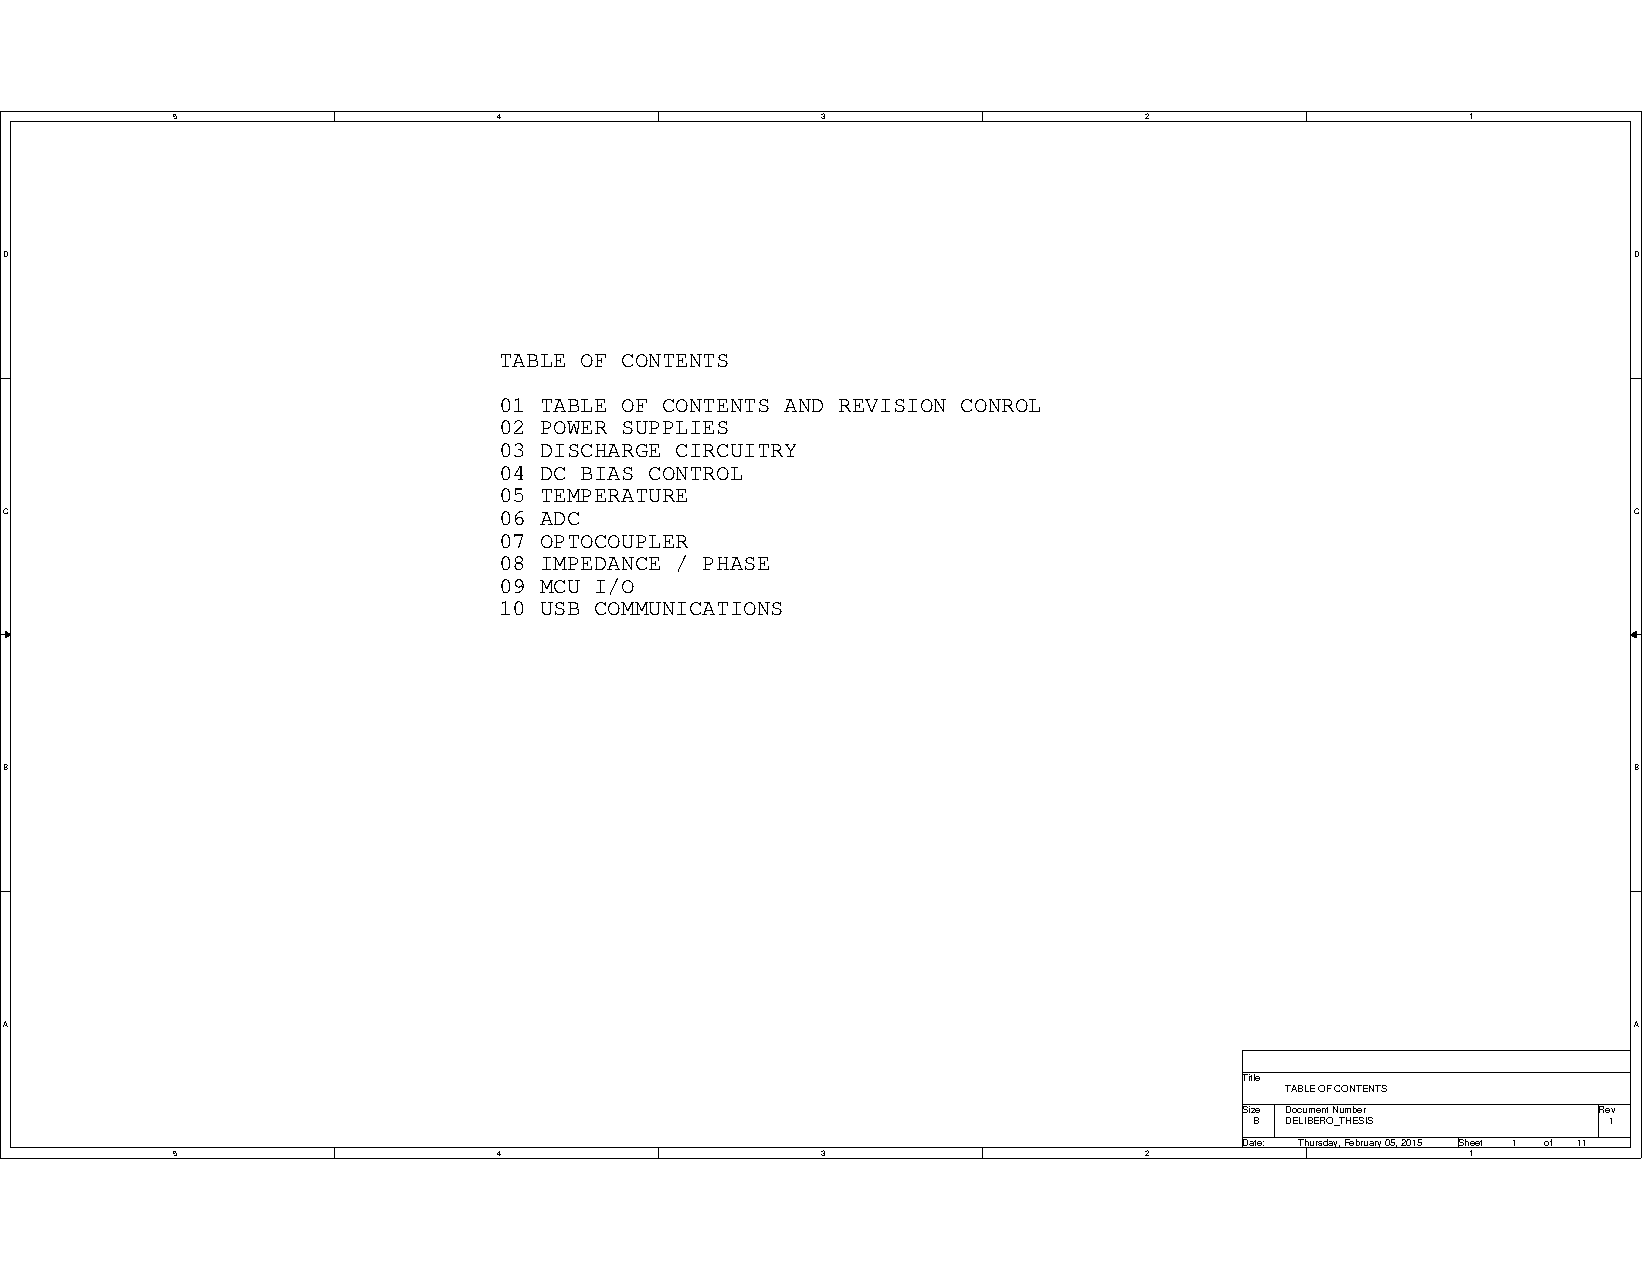
\includepdf[pages=-,angle=90,rotateoversize,offset=1.75in -.975in]{figures/board/capMeasCircuit.pdf}

\section{Generating Modeling Images}
\label{app:genModelingImages}
This appendix will list all of the matlab code and supporting files needed to generate the images seen in Section: \ref{sec:regression}.

\subsection{Example Data: Figure: \ref{fig:exCapData}}
\begin{figure}[ht!]
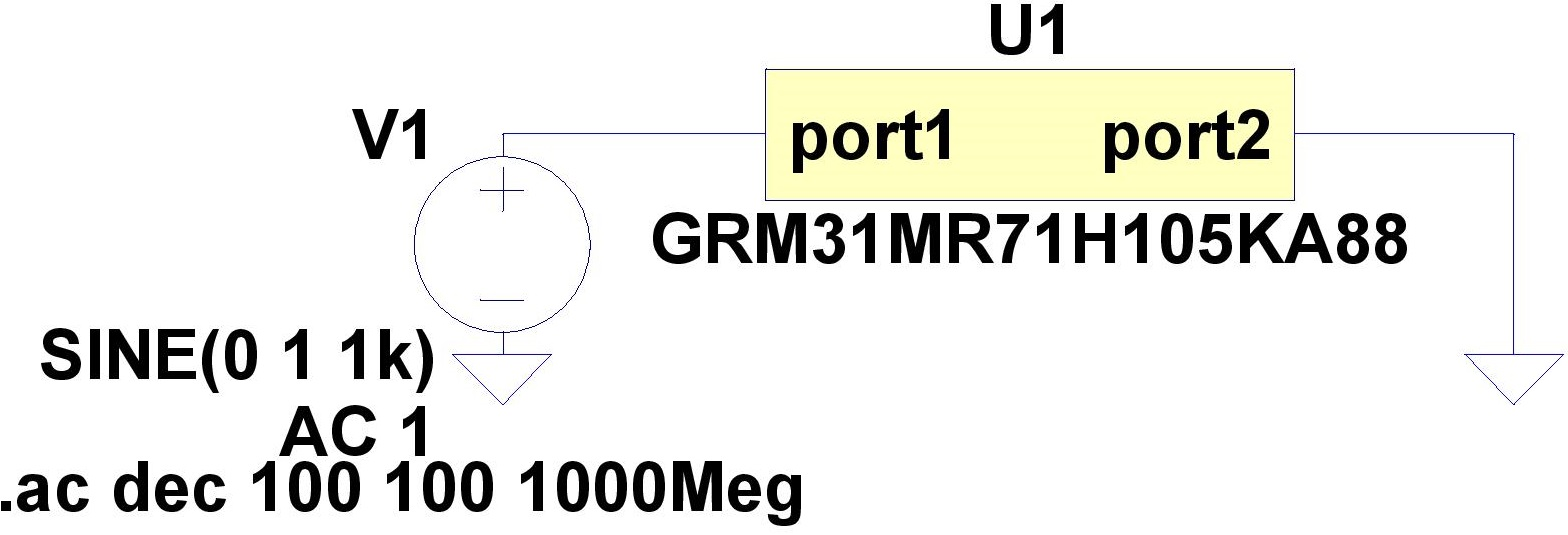
\includegraphics[keepaspectratio=true,width=2in]{./figures/appendix/exCapData_ltspice.jpg}
\centering
\caption{LTSpice Schematic for Capacitor Model}
\label{fig:exCapData_ltspice}
\end{figure}


This section will describe how to obtain and generate the example data used for the regression fitting. This method uses LTSpice to generate impedance vs frequency data from one of Murata's capacitor models. First, go to Murata's online SimSurfing tool \cite{simSurfing} and select the ``Monolithic Ceramic Capacitors'' button. Download a SPICE *.mod file (Appendix: \ref{app:subcir}) for the capacitor of interest, by selecting it from the list and clicking the ``netlist'' button. Open the *.mod file in LTSpice, right click on the part name in the line starting with ``.SUBCKT,'' and select ``Create Symbol.'' Create an LTSpice schematic similar to Figure: \ref{fig:exCapData_ltspice} and plot $\frac{V(n001)}{-I(V1)}$. The negative sign is important because LTSpice defines current as coming out of a node. If the negative sign is omitted, the phase will be offset by $180^o$, and the regression analysis will solve for negative capacitance! With the plot window selected, select  $``File\rightarrow Export\rightarrow Cartesian\rightarrow OK$'' with the impedance plot selected as the waveform. Open the resultant *.txt file, delete the first line, and change all tabs to commas (``$<:>\%s/<ctrl+v><TAB>/,/g$'' , ``$\%s/\string^I/,/g$'' in vim). Make sure to save the resultant file in ``/scripts/data.''

\subsubsection{Capacitor Subcircuit Model}
\label{app:subcir}
\lstinputlisting{./scripts/data/GRM31MR71H105KA88.mod}

\subsubsection{Plot ExCapData Script}
The functions used to get and plot the data can be found in Appendix: \ref{app:utilityFuns}.
\lstinputlisting{./scripts/regression/plot_ExCapData.m}

\subsection{Basic LSE Image: Figure: \ref{fig:basicLSE}}
\lstinputlisting{./scripts/regression/run_basicLSE.m}

\subsection{Levy's Method: Figures: \ref{fig:levy}, \ref{fig:levyIter_Err1}, \ref{fig:levyIter_Err2}, \& \ref{fig:levyIter}}
\lstinputlisting{./scripts/regression/run_levy_iter.m}
\lstinputlisting{./scripts/getInitGuess.m}
\lstinputlisting{./scripts/regression_levy_iter.m}

\subsection{Utility Functions}
\label{app:utilityFuns}
This appendix holds common ``utility'' functions used by many of the MATLAB scripts. You are required to manually save each plot after calling the ''plotfit.m.''

\lstinputlisting{./scripts/utilityFuns/getData.m}
\lstinputlisting{./scripts/utilityFuns/plotFit.m}
\lstinputlisting{./scripts/utilityFuns/plotType.m}


\section{Additional Regression Techniques}
\label{app:adtl_regression}
\nocite{neu_ModelSynth}
\nocite{cuth_regression}
\nocite{bbc_chebyshev}

% Run /scripts/appendix/powerSeries.m
\begin{figure}[ht!]
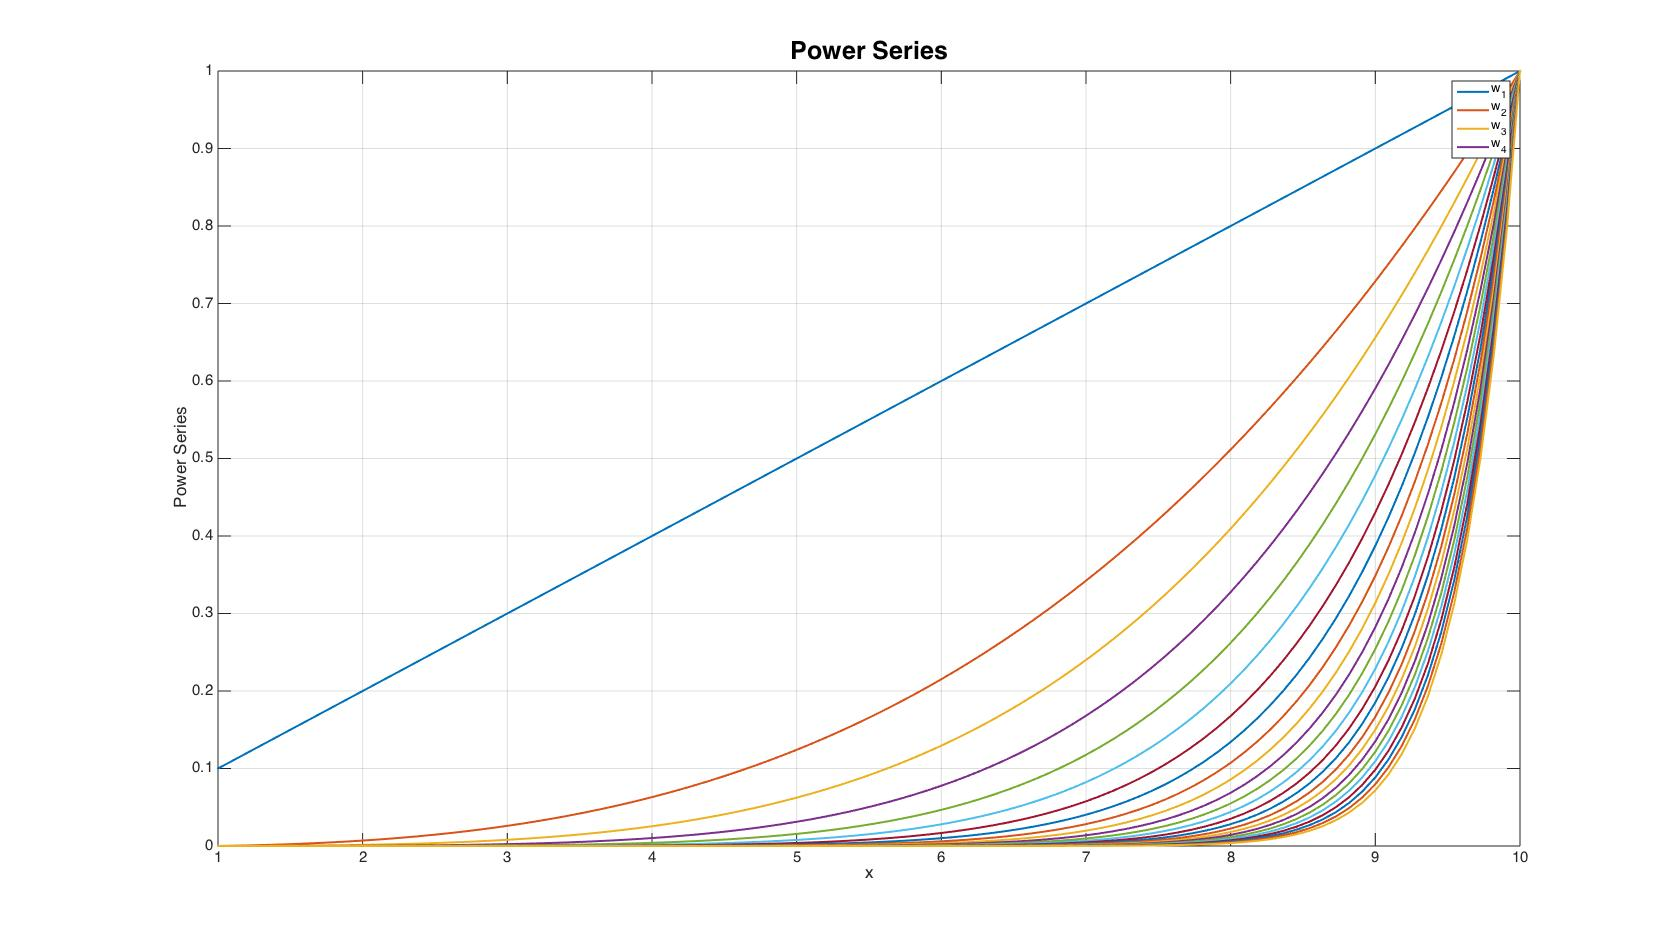
\includegraphics[keepaspectratio=true,width=6in]{./figures/appendix/powerSeries.jpg}
\centering
\caption{Power Series \cite{beyene_uwave}[Fig: 1]}
\label{fig:powerSeries}
\end{figure}



This section will cover the theory behind a computational method that should improve the results obtained in Section: \ref{sec:regression}. As previously stated, the main problem with applying Levy's approach to capacitor modeling is that it is ill-suited for wide bandwidth applications. As stated by Beyene, ``this is because the ordinary power series ${\omega ^0, \omega ^1, \omega ^2, \omega ^3,...}$ have a large dynamic range, and they become almost parallel at higher orders. As show in Figure: \ref{fig:powerSeries}, for higher orders, the shapes of the power series become very similar over most of the normalized frequency range. \cite{beyene_uwave}''

\begin{equation}
\label{equ:cheby}
T_{n+1} = 2xT_{n}-T_{n-1}
\end{equation}

\begin{equation}
    \label{equ:chebyPolys}
    \begin{split}
         T_0(x) &= 1           \\
         T_1(x) &= x           \\
         T_2(x) &= 2x^2-1      \\
         T_3(x) &= 4x^3-3x     \\
         T_4(x) &= 8x^4-8x^2+1 \\
         T_5(x) &= 16x^5-20x^3+5x
    \end{split}
\end{equation}

The proposed methodology uses Chebyshev polynomials of the first kind to circumvent this problem. As seen in Equation: \eqref{equ:cheby}, they are recursively defined with $T_0 = 1$ and $T_1 = x$. This results in polynomials that are orthogonal over a normalized frequency range, as seen in Figure: \ref{fig:cheby}. Gao\cite{gao_blackBox} shows that the frequency terms in an LSE can be replaced with Chebyshev polynomials. The coefficients found via this method are not the same as the coefficients in the frequency space. One needs to use Clenshaw's Recurrence Formula \cite{gao_blackBox}[Equation: 11] in order to get the desired coefficients. This method should produce a result that is more accurate due to its avoidance of the ill-conditioned matrix while solving the system of equations.

% Run /scripts/appendix/cheby.m
\begin{figure}[ht!]
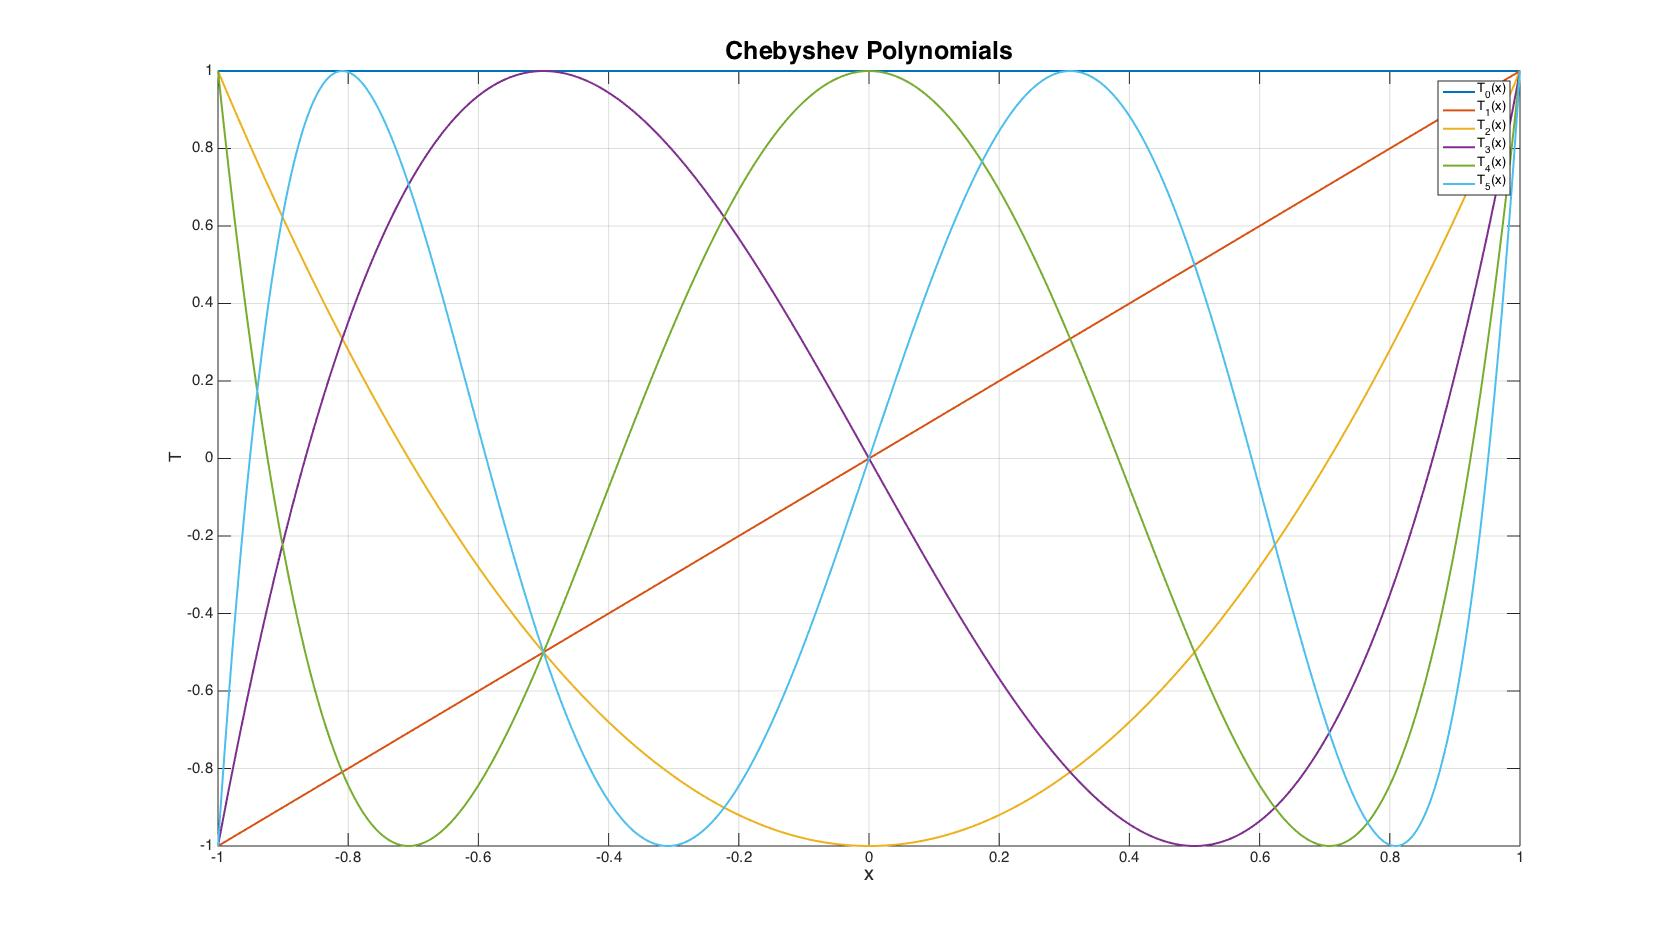
\includegraphics[keepaspectratio=true,width=6in]{./figures/appendix/cheby.jpg}
\centering
\caption{Chebyshev Polynomials \cite{wolf_cheby}}
\label{fig:cheby}
\end{figure}







\bibliography{metadata/thesis,figures/thesis_figs}
\end{document}

